\chapter{Laboratorio 1}

%%%%%%%%%%%%%%%%%%%%%%%%%%%%%%%%%%%%%%%%%%%%%%%%%%%%%%%%%%%

%%%%%%   Primo esercizio --------------------------------------
\section{Modi guidati di una guida d'onda slab SOI}
L'obiettivo del primo Assignment del Laboratorio 1 è lo studio di una guida Slab realizzata con tecnologia SOI e simulata numericamente con i seguenti parametri fisici:

\begin{itemize}
    \item Indice di rifrazione del core: $\boldsymbol{n_{Si} = n_{1} = 3.48}$
    \item Indice di rifrazione del cladding: $\boldsymbol{n_{SiO_2} = n_{2} = 1.44}$
    \item Lunghezza d'onda della luce: $\boldsymbol{\lambda = 1.31 \, \mu m}$
\end{itemize}

\subsection{Calcolo di $\boldsymbol{n_{eff}}$ in funzione di $\boldsymbol{d}$}

\noindent I possibili valori dell'indice di rifrazione efficace $n_{eff}$, in funzione della larghezza dello slab $d$, sono riportati in Figura \ref{fig:neff_vs_d}, ricavati tramite l'equazione \ref{eq:d}

\begin{equation}\label{eq:d}
    d = \frac{tan^{-1}(\frac{\gamma}{k_x}) + tan^{-1}(\frac{\delta}{k_x}) + m\pi}{k_x}
\end{equation}

\begin{figure}[!h]
 \centering
 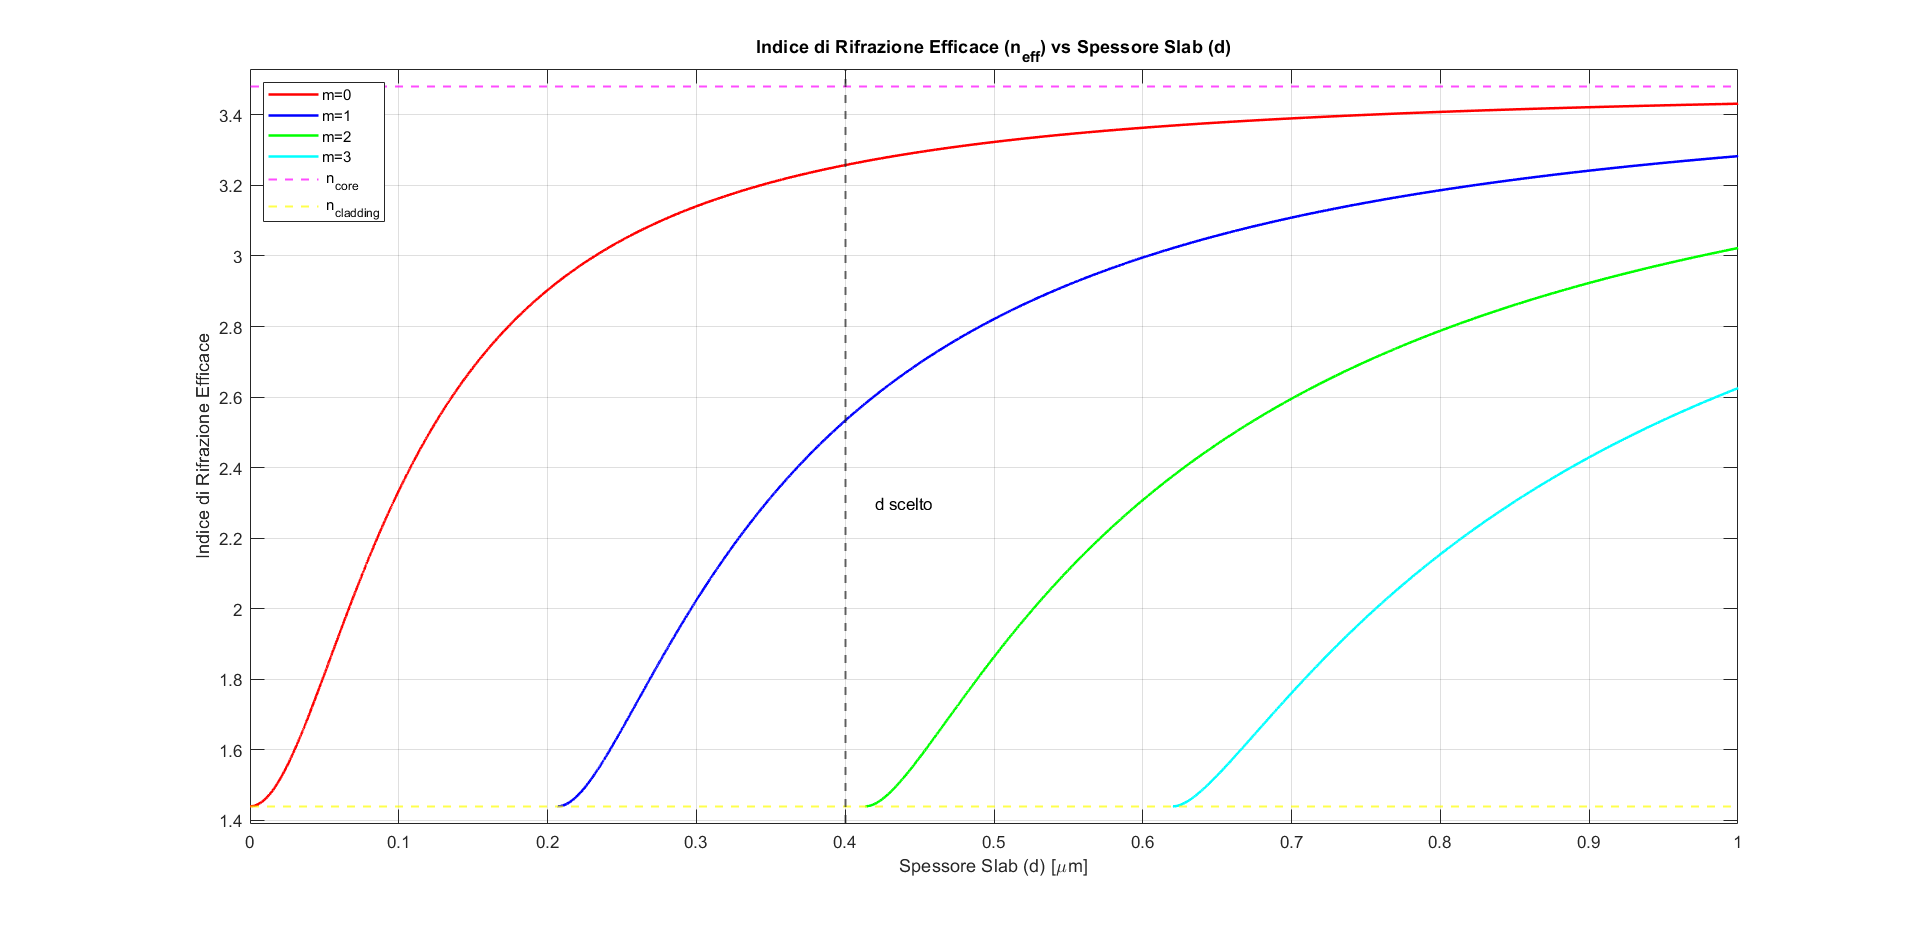
\includegraphics[width=15cm]{lab1/Images/prob1/neff_vs_d.png}
  \caption{Plot di $n_{eff}$ in funzione di $d$ per i primi 4 modi guidati}
  \label{fig:neff_vs_d}
\end{figure}

\noindent I termini $\gamma$, $\delta$ e $k_{x}$ sono tutti dipendenti da $n_{eff}$ secondo le relazioni riportate di seguito:

\begin{equation}
    k_x = \sqrt{k_0^2 n_1^2 - \beta^2} = k_0 \cdot \sqrt{n_1^2 - n_{eff}^2}
\end{equation}

\begin{equation}
    \gamma = \delta = \sqrt{\beta^2 - k_0^2 n_2^2} = k_0 \cdot \sqrt{n_{eff}^2 - n_2^2}
\end{equation}

\noindent Dal grafico \ref{fig:neff_vs_d} si evince che alla larghezza $d \approx 0.21 \,\mu m$ la guida passa dal propagare il solo modo fondamentale $TE_0$
al diventare una guida multimodale, in quanto propaga anche il primo modo superiore $TE_1$. Scegliendo un valore di $d$ congruo, si può ottenere una guida che 
permetta esclusivamente la propagazione dei primi due modi ($ 0.21 \mu m < d < 0.41 \mu m$). 

\subsection{Plot dei campi elettromagnetici}
Dopo aver scelto un valore di $d$ che permetta la propagazione dei primi due modi guidati (denominato $\boldsymbol{d_{scelto} = 0.4 \mu m}$), è possibile plottare
le distribuzioni di campo elettrico e magnetico relativi ai modi $TE_0$ e $TE_1$.\\
\noindent\\ Le intensità dei campi (ossia il loro modulo al quadrato $|E_y|^2$, $|H_x|^2$ e $|H_z|^2$) sono riportate
nelle Figure \ref{fig:I_Ey}, \ref{fig:I_Hx} e \ref{fig:I_Hz}.

\begin{figure}[!h]
 \centering
 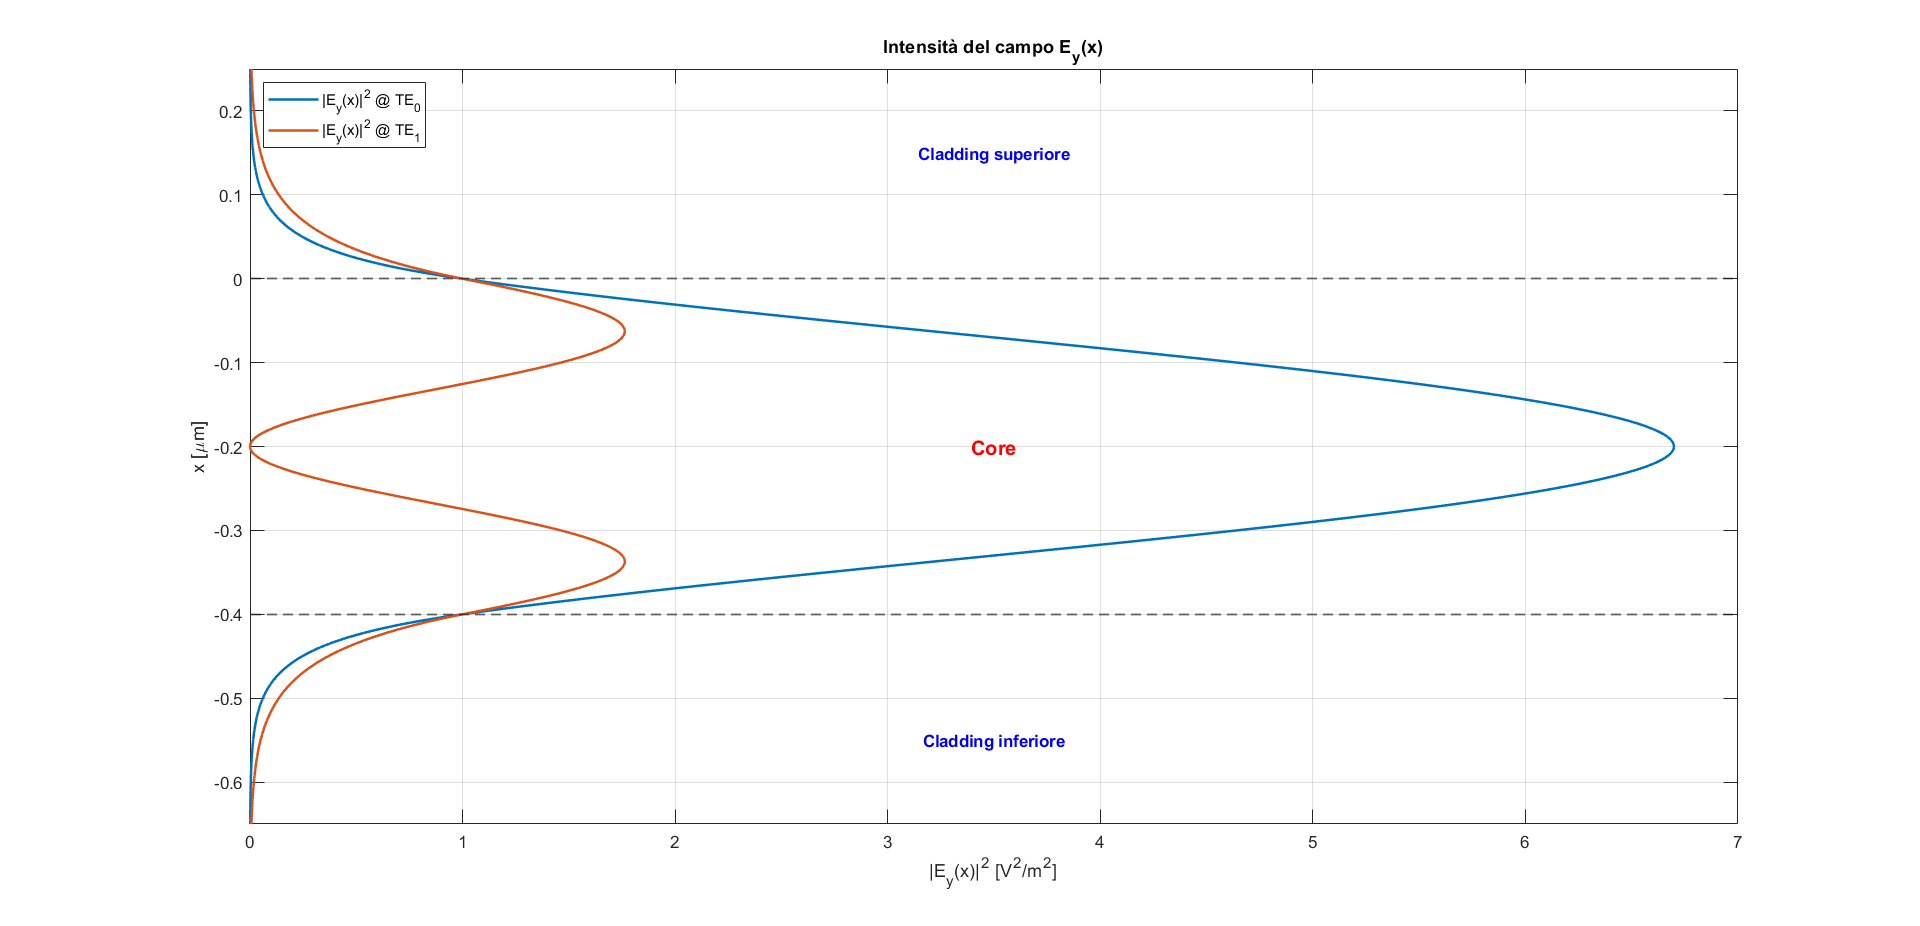
\includegraphics[width=15cm]{lab1/Images/prob1/I_Ey.png}
  \caption{Intensità del campo elettrico $E_y$ per i modi $TE_0$ e $TE_1$}
  \label{fig:I_Ey}
\end{figure}

\begin{figure}[!h]
 \centering
 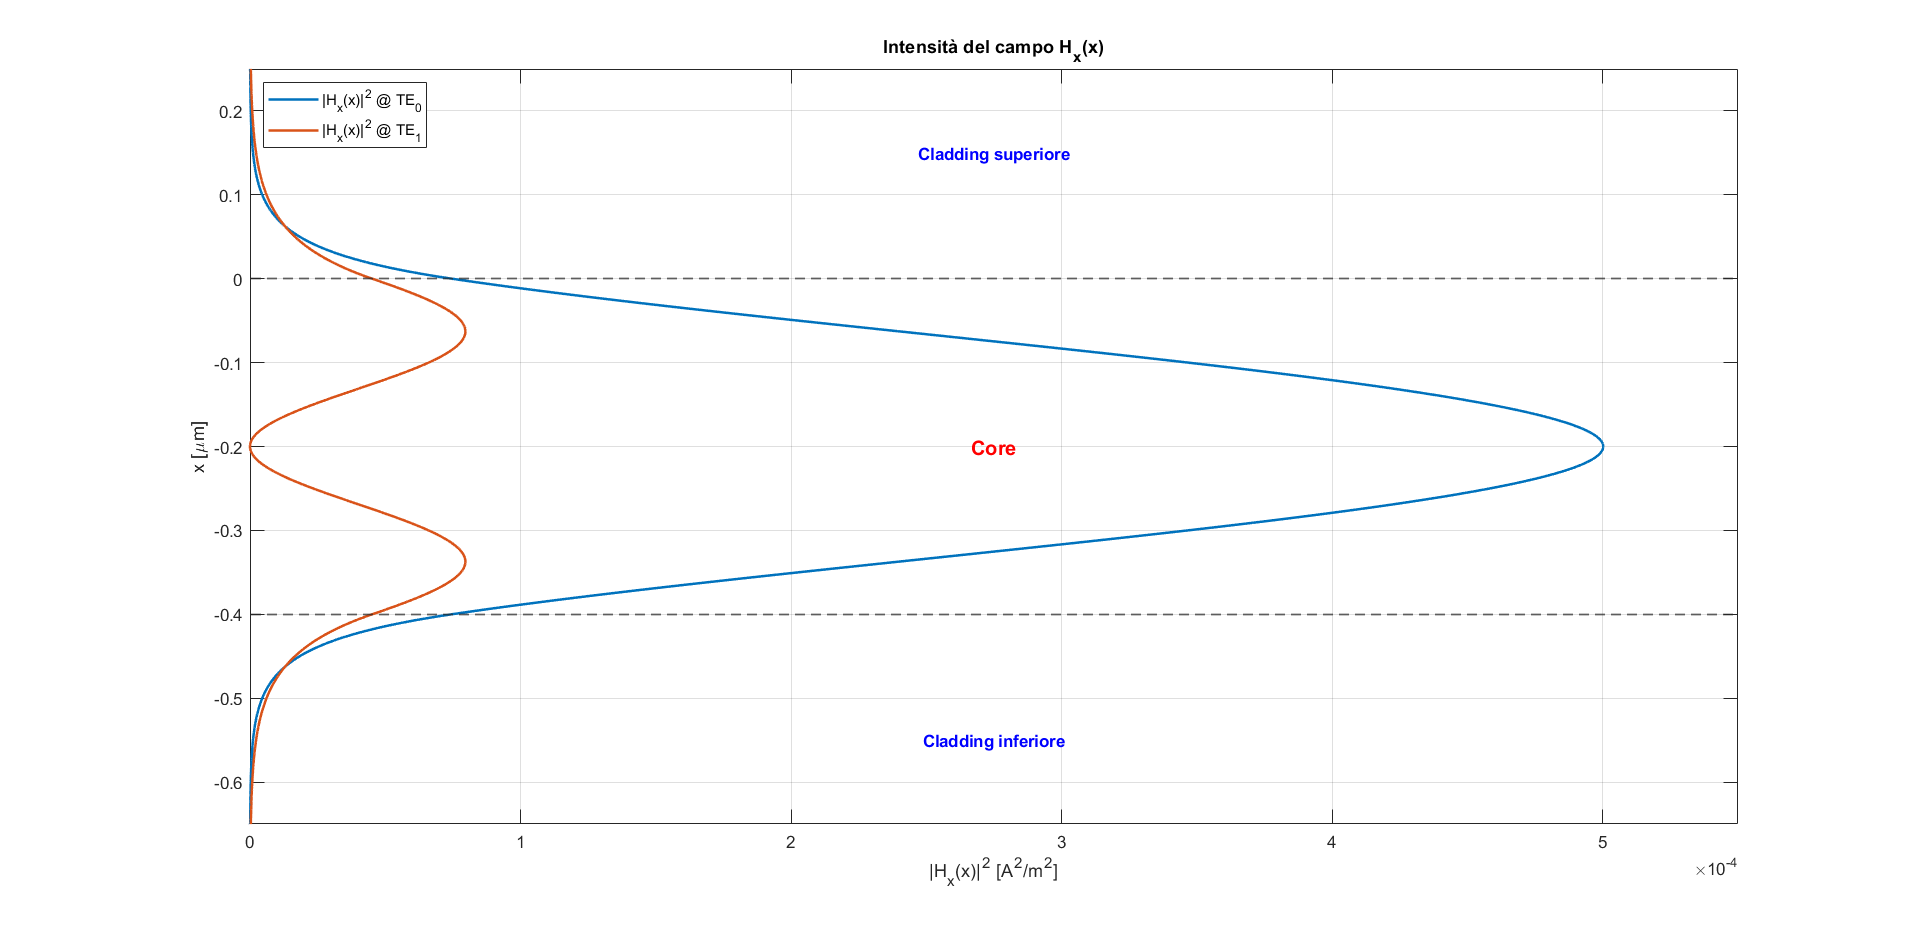
\includegraphics[width=15cm]{lab1/Images/prob1/I_Hx.png}
  \caption{Intensità del campo magnetico $H_x$ per i modi $TE_0$ e $TE_1$}
  \label{fig:I_Hx}
\end{figure}

\begin{figure}[!h]
 \centering
 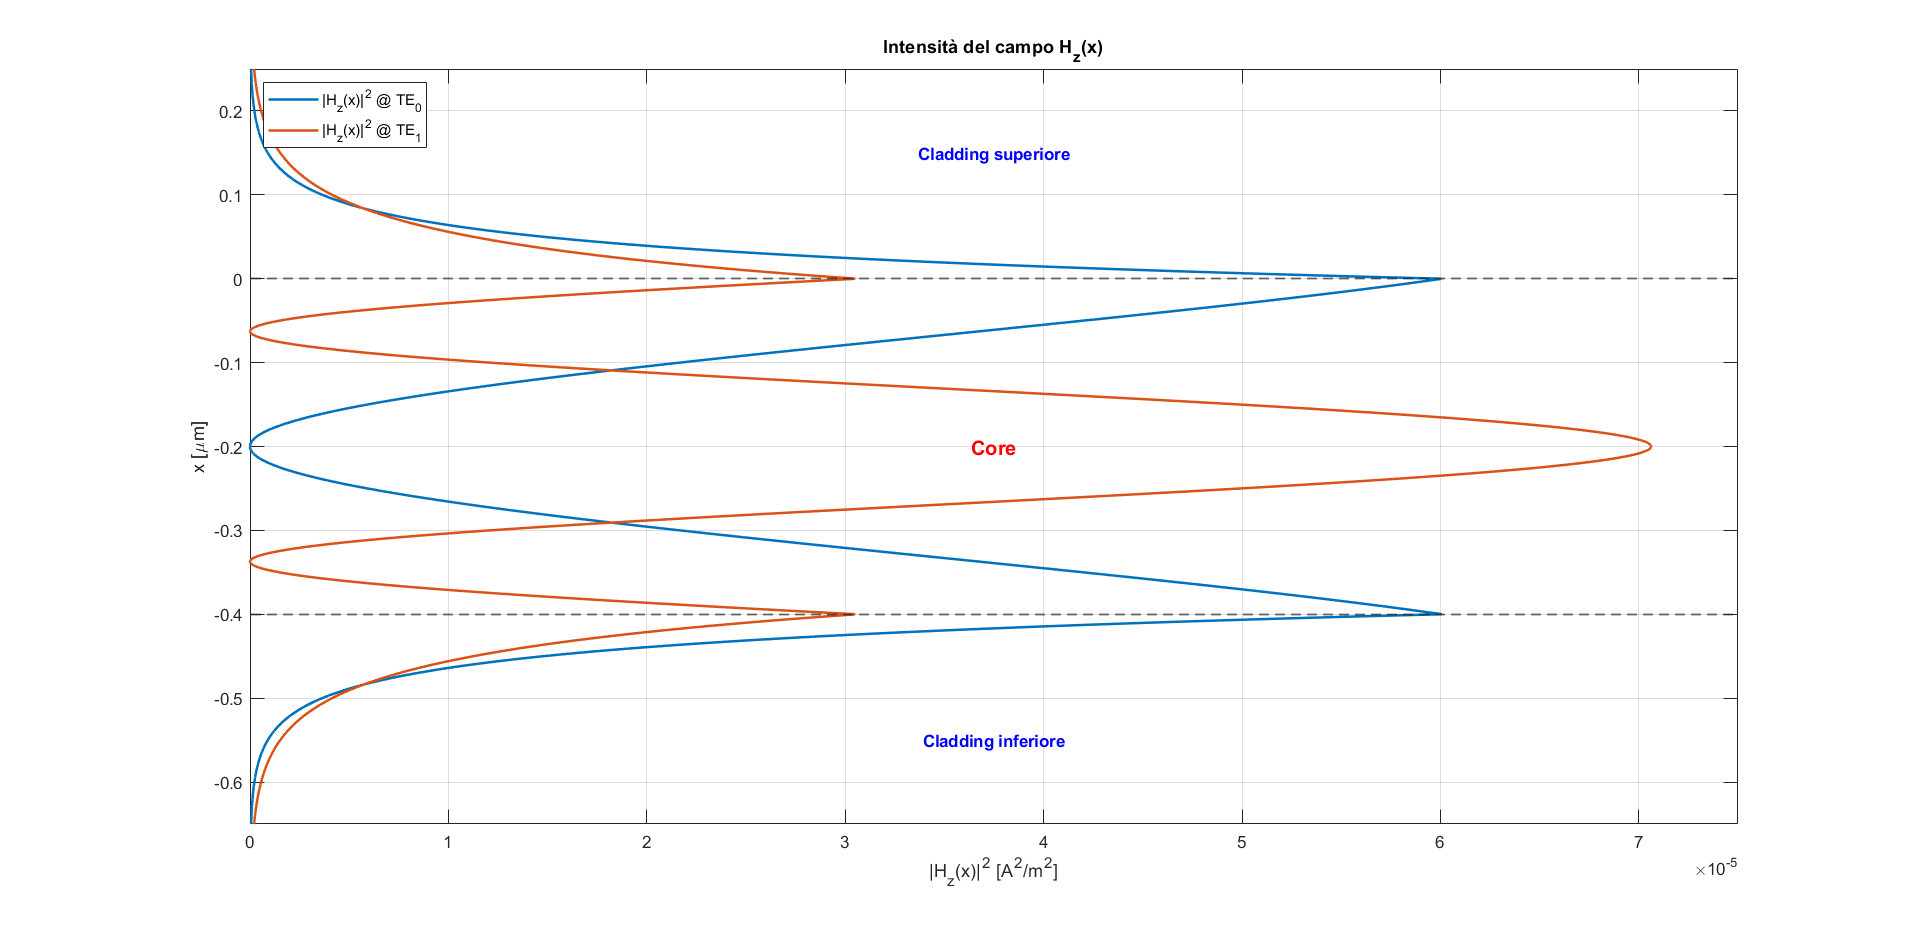
\includegraphics[width=15cm]{lab1/Images/prob1/I_Hz.png}
  \caption{Intensità del campo magnetico $H_z$ per i modi $TE_0$ e $TE_1$}
  \label{fig:I_Hz}
\end{figure}

\newpage
\noindent Per quanto riguarda il campo elettrico, la sua espressione è stata calcolata analiticamente dalle equazioni di Maxwell, imponendo che la componente lungo
l'asse di propagazione fosse nulla (ossia $E_z = 0$) e che non ci fossero variazioni delle componenti lungo l'asse y (ossia $\frac{\partial F}{\partial y} = 0$,
con $F$ che rappresenta una generica componente di un campo). Inoltre, è stata imposta la condizione di continuità alle interfacce tra core e cladding
(ovvero alle coordinate $x = 0$ e $x = -d$). L'espressione a tratti del campo elettrico risultante è riportata di seguito:

\begin{equation}
    E_y(x) = \begin{cases}
        A\cdot e^{-\delta x} & \text{per } x > 0 \\
        A\cdot cos(k_x \cdot x) + B \cdot sin(k_x \cdot x) & \text{per } -d < x < 0 \\
        [A\cdot cos(k_x \cdot d) - B \cdot sin(k_x \cdot d)] \cdot e^{\gamma (x+d)} & \text{per } x < -d
    \end{cases}
\end{equation}

\noindent\\ È importante evidenziare come la scelta di un opportuno valore di $d$ sia fondamentale, in primis per garantire la propagazione dei soli modi
desiderati, evitando la presenza di modi superiori, ma anche per la definizione del valore dell'indice di rifrazione efficace $n_{eff}$, che a sua volta
influenza il profilo dei campi, tramite le grandezze $k_x$, $\gamma$ e $\delta$.\\
Con il valore di $d$ scelto, i valori di $n_{eff}$ risultanti per i modi $TE_0$ e $TE_1$ sono rispettivamente:
\[
 \boldsymbol{n_{eff,TE_0} = 3.26} \,\,\,\,\,\,\,\, \text{,} \,\,\,\,\,\,\,\, \boldsymbol{n_{eff,TE_1} = 2.53}
\]

\noindent\\ Per quanto riguarda i campi magnetici, le loro espressioni sono state calcolate a partire dal campo elettrico, tramite le equazioni di Maxwell.
In particolare, le espressioni che rappresentano i campi magnetici risultanti sono riportate di seguito:

\begin{equation}
    H_x(x) = -\frac{\beta}{\omega\cdot \mu_0} \cdot E_y(x) = -\frac{n_{eff}}{c\cdot\mu_0} \cdot E_y(x)
\end{equation}

\begin{equation}
    H_z(x) = j\frac{1}{\omega\cdot \mu_0} \cdot \frac{\partial E_y(x)}{\partial x}
\end{equation}

\noindent\\ Imponendo le condizioni di continuità alle interfacce tra core e cladding anche per i campi magnetici, si ottiene l'espressione che lega le
costanti $A$ e $B$ del campo elettrico e l'equazione trascendente utilizzata in precedenza, che lega $n_{eff}$ e $d$:

\begin{equation}
    \frac{B}{A} = -\frac{\delta}{k_x}
\end{equation}

\begin{equation}
    tan(k_x \cdot d) = \frac{k_x\cdot(\gamma+\delta)}{k_x^2 - \gamma\cdot\delta}
\end{equation}

%, le quali a loro volta dipendono
%da $n_{eff}$. La scelta di un valore di $d$ troppo grande potrebbe portare alla propagazione di modi superiori, mentre un valore troppo piccolo
%potrebbe non permettere la propagazione nemmeno del modo fondamentale. Inoltre, la larghezza dello slab influenza anche la distribuzione dei campi
%elettromagnetici all'interno della guida, determinando la forma delle intensità dei campi elettrico e magnetico. Infine, è importante considerare che
%la presenza di imperfezioni o disomogeneità nella guida d'onda può causare scattering o perdite di potenza,
%che potrebbero interferire con le prestazioni della guida d'onda. 

\newpage
\subsection{Calcolo del Fattore di Confinamento Ottico (OCF) $\boldsymbol{\Gamma_{TE_0}}$}
Focalizzandosi solamente sul modo $TE_0$, si è calcolata analiticamente, al variare dello spessore dello slab $d$, l'espressione
del Fattore di Confinamento Ottico nel core $\Gamma_{TE_0}$. Questo valore indica quanto la luce sia effettivamente confinata nel core, infatti è 
definito come il rapporto tra la potenza confinata nel core e la potenza totale.
\begin{equation}
    \Gamma_{TE_0} = \frac{P_{core}}{P_{totale}} = \frac{\int_{-d}^{0} |E_y(x)|^2 dx}{\int_{-\infty}^{+\infty} |E_y(x)|^2 dx}
\end{equation}

\noindent\\ L'andamento del Fattore di Confinamento Ottico $\Gamma_{TE_0}$ in funzione dello spessore dello slab $d$ è riportato in Figura \ref{fig:Gamma_vs_d}.

\begin{figure}[!h]
 \centering
 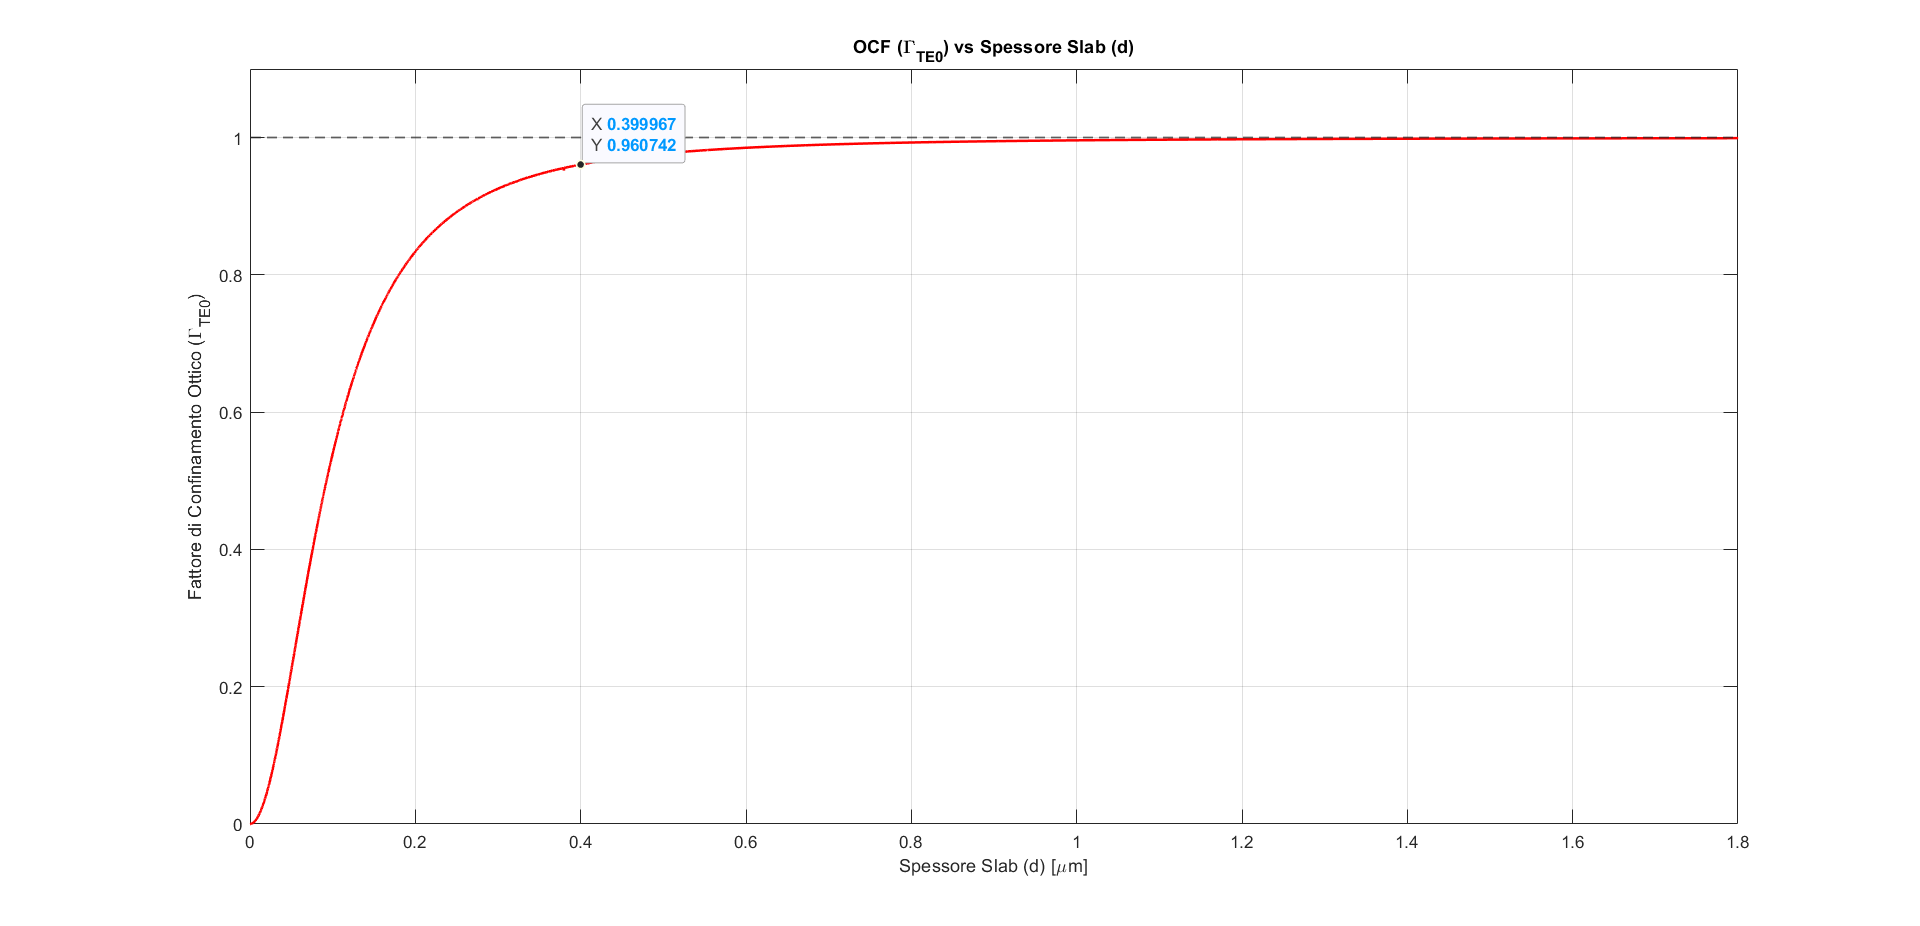
\includegraphics[width=15cm]{lab1/Images/prob1/Gamma_vs_d.png}
  \caption{Plot di $\Gamma_{TE_0}$ in funzione di $d$ per il modo $TE_0$}
  \label{fig:Gamma_vs_d}
\end{figure}

\noindent Dal grafico si evince come il fattore di confinamento ottico $\Gamma_{TE_0}$ aumenti al crescere dello spessore dello slab $d$,
raggiungendo valori prossimi all'unità per $d \approx 0.8 \mu m$. Questo significa che, per spessori maggiori di $0.8 \mu m$, la maggior
parte della potenza del modo $TE_0$ è confinata nel core della guida, mentre per spessori (molto) minori di $0.8 \mu m$ una parte significativa
della potenza potrebbe disperdersi nel cladding, riducendo l'efficienza della guida.\\
\noindent\\ Con lo spessore inizialmente scelto ($d_{scelto} = 0.4 \mu m$)
per avere solo i primi due modi, il fattore di confinamento ottico risulta essere $\Gamma_{TE_0} \cong 0.96$, ossia circa il 96\% della potenza
del modo $TE_0$ è confinata nel core della guida, quindi solamente il 4\% della potenza modale è localizzata nel cladding.


\newpage

\subsection{Calcolo del Modal Loss $\boldsymbol{\alpha_{modal}}$}

Successivamente si è proceduto a calcolare anche l'Attenuazione Modale (\textit{Modal Loss}) per il modo $TE_0$, tenendo conto sia
dell'attenuazione nel core ($\alpha_{core} = \alpha_{Si}$) e nel cladding ($\alpha_{cladding} = \alpha_{SiO_2}$).
Il Modal Loss è definito dalla seguente espressione:

\begin{equation}
    \alpha_{modal} = \Gamma_{core} \cdot \alpha_{core} + \Gamma_{cladding} \cdot \alpha_{cladding}
\end{equation}

\noindent\\ dove $\Gamma_{core} = \Gamma_{TE_0}$ è uguale al Fattore di Confinamento Ottico calcolato in precedenza,
mentre $\Gamma_{cladding} = 1 - \Gamma_{TE_0}$ è il complementare di $\Gamma_{core}$.
\noindent\\\\ Il Modal Loss è stato calcolato al variare dello spessore dello slab $d$, riportandolo sia
in $cm^{-1}$ che in $dB/cm$, come mostrato nelle Figure \ref{fig:amod_cm_vs_d} e \ref{fig:amod_db_vs_d}.

\begin{figure}[!h]
 \centering
 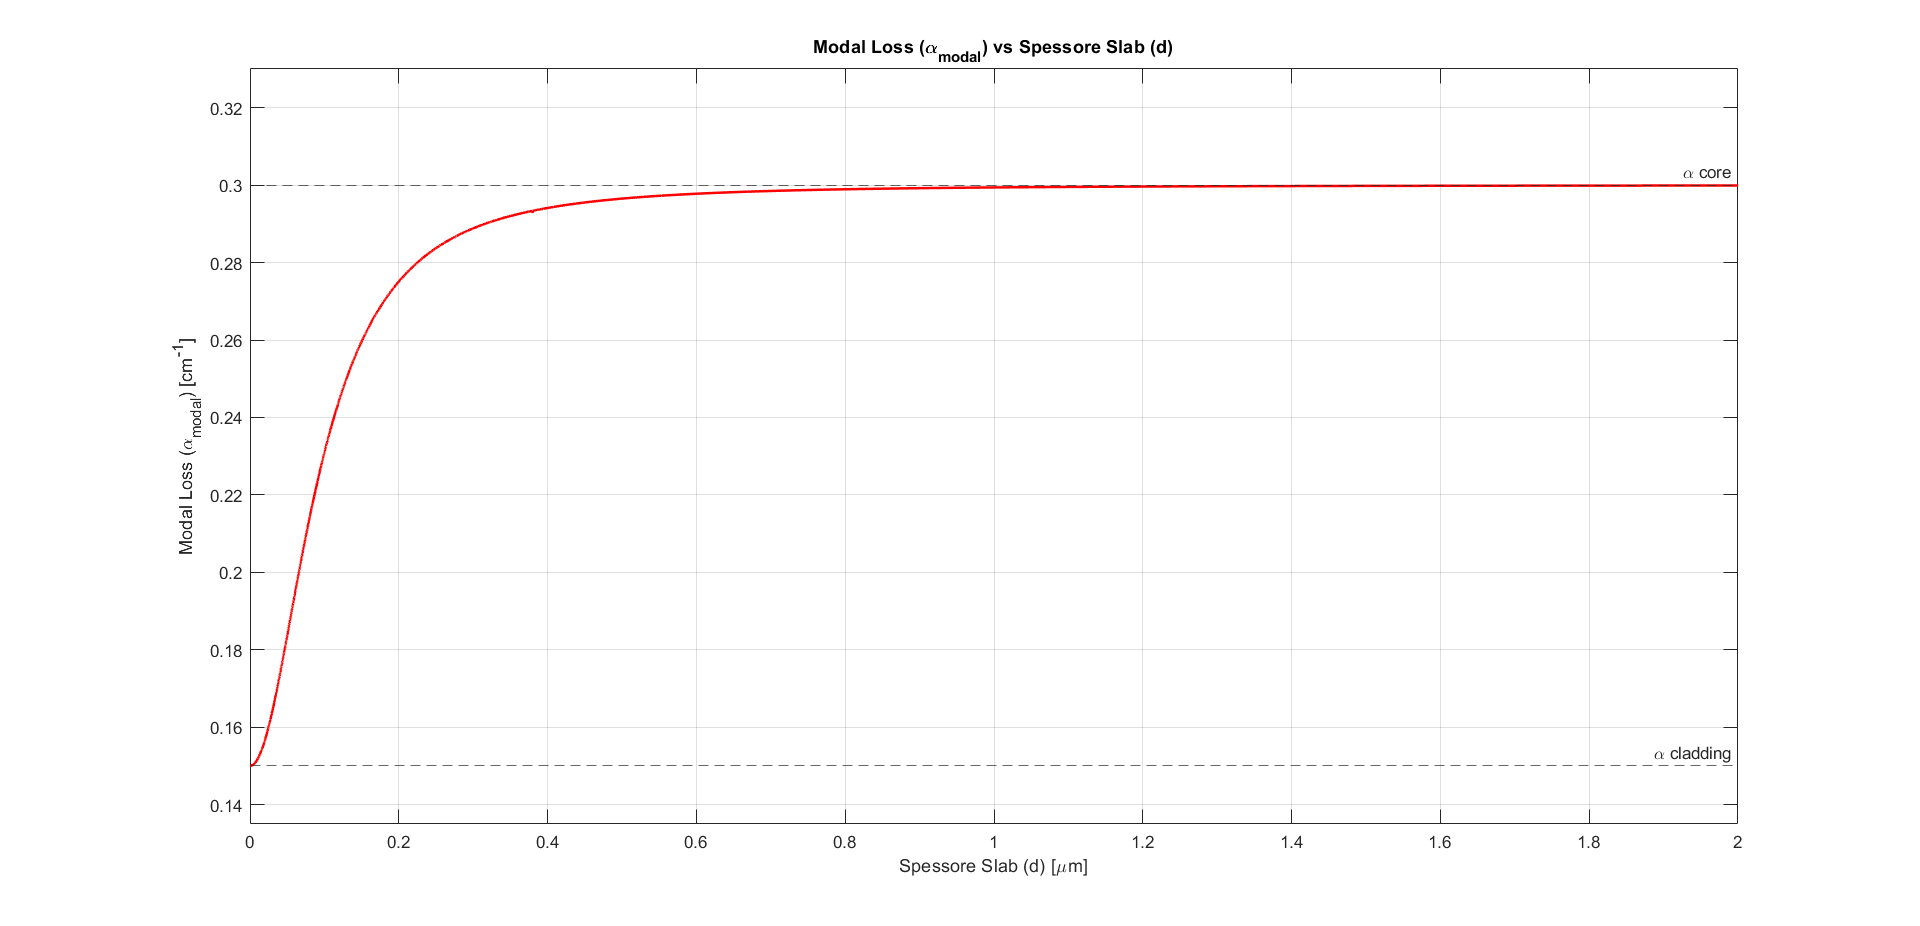
\includegraphics[width=15cm]{lab1/Images/prob1/a_mod_cm.png}
  \caption{Plot di $\alpha_{modal}$ [cm$^{-1}$] in funzione di $d$ per il modo $TE_0$}
  \label{fig:amod_cm_vs_d}
\end{figure}

\begin{figure}[!h]
 \centering
 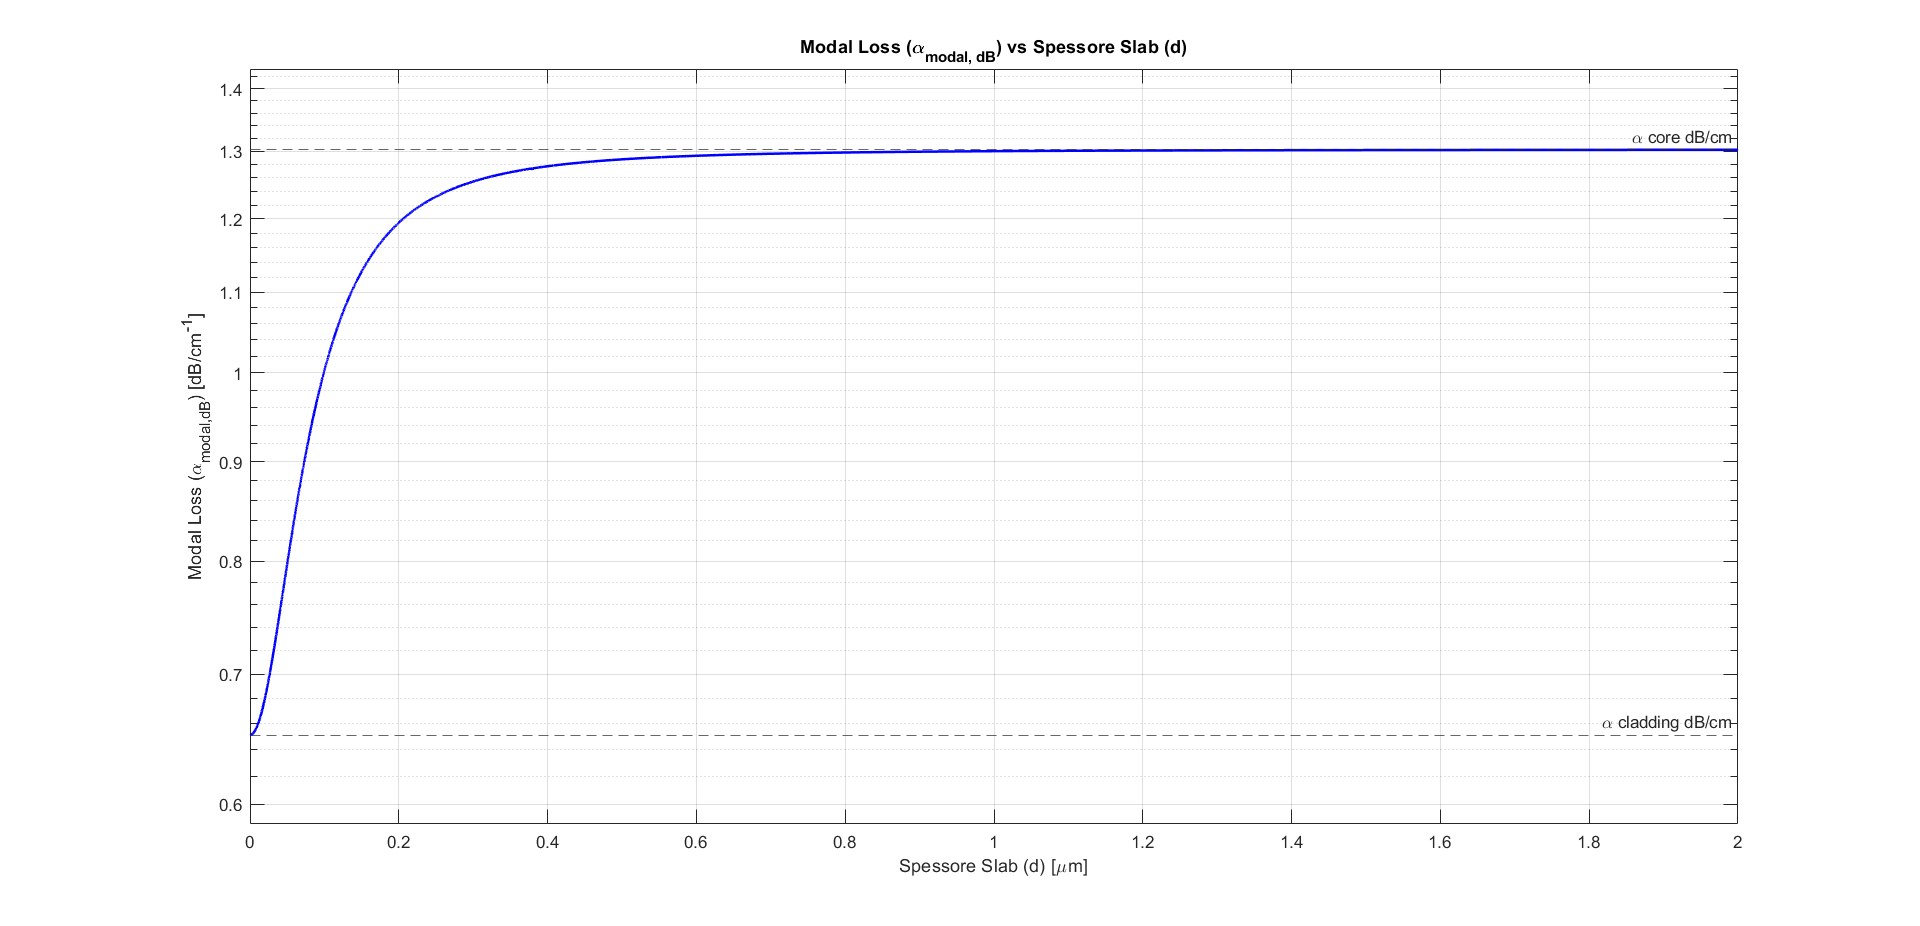
\includegraphics[width=15cm]{lab1/Images/prob1/a_mod_db.png}
  \caption{Plot di $\alpha_{modal}$ [dB/cm] in funzione di $d$ per il modo $TE_0$}
  \label{fig:amod_db_vs_d}
\end{figure}

\newpage
\subsection{Calcolo dell'Insertion Loss $\boldsymbol{IL_{dB}}$}

Considerando che la guida sia lunga ($L = 5 \, mm = 0.5 \, cm$), si è calcolato l'Insertion Loss in dB,
ossia la perdita di potenza dovuta alla propagazione del modo $TE_0$ lungo la guida.\\
L'Insertion Loss è definito dalla seguente espressione:
\begin{equation}
    IL_{dB} = \alpha_{modal,dB} \cdot L
\end{equation}

\noindent dove $\alpha_{modal,dB}$ è il Modal Loss (in dB/cm) calcolato in precedenza,
mentre $L$ è la lunghezza della guida in cm. Anche in questo caso, il risultato è stato
rappresentato graficamente (Figura \ref{fig:IL_vs_d}) per visualizzare la variazione delle perdite 
totali in funzione dello spessore d.

\begin{figure}[!h]
 \centering
 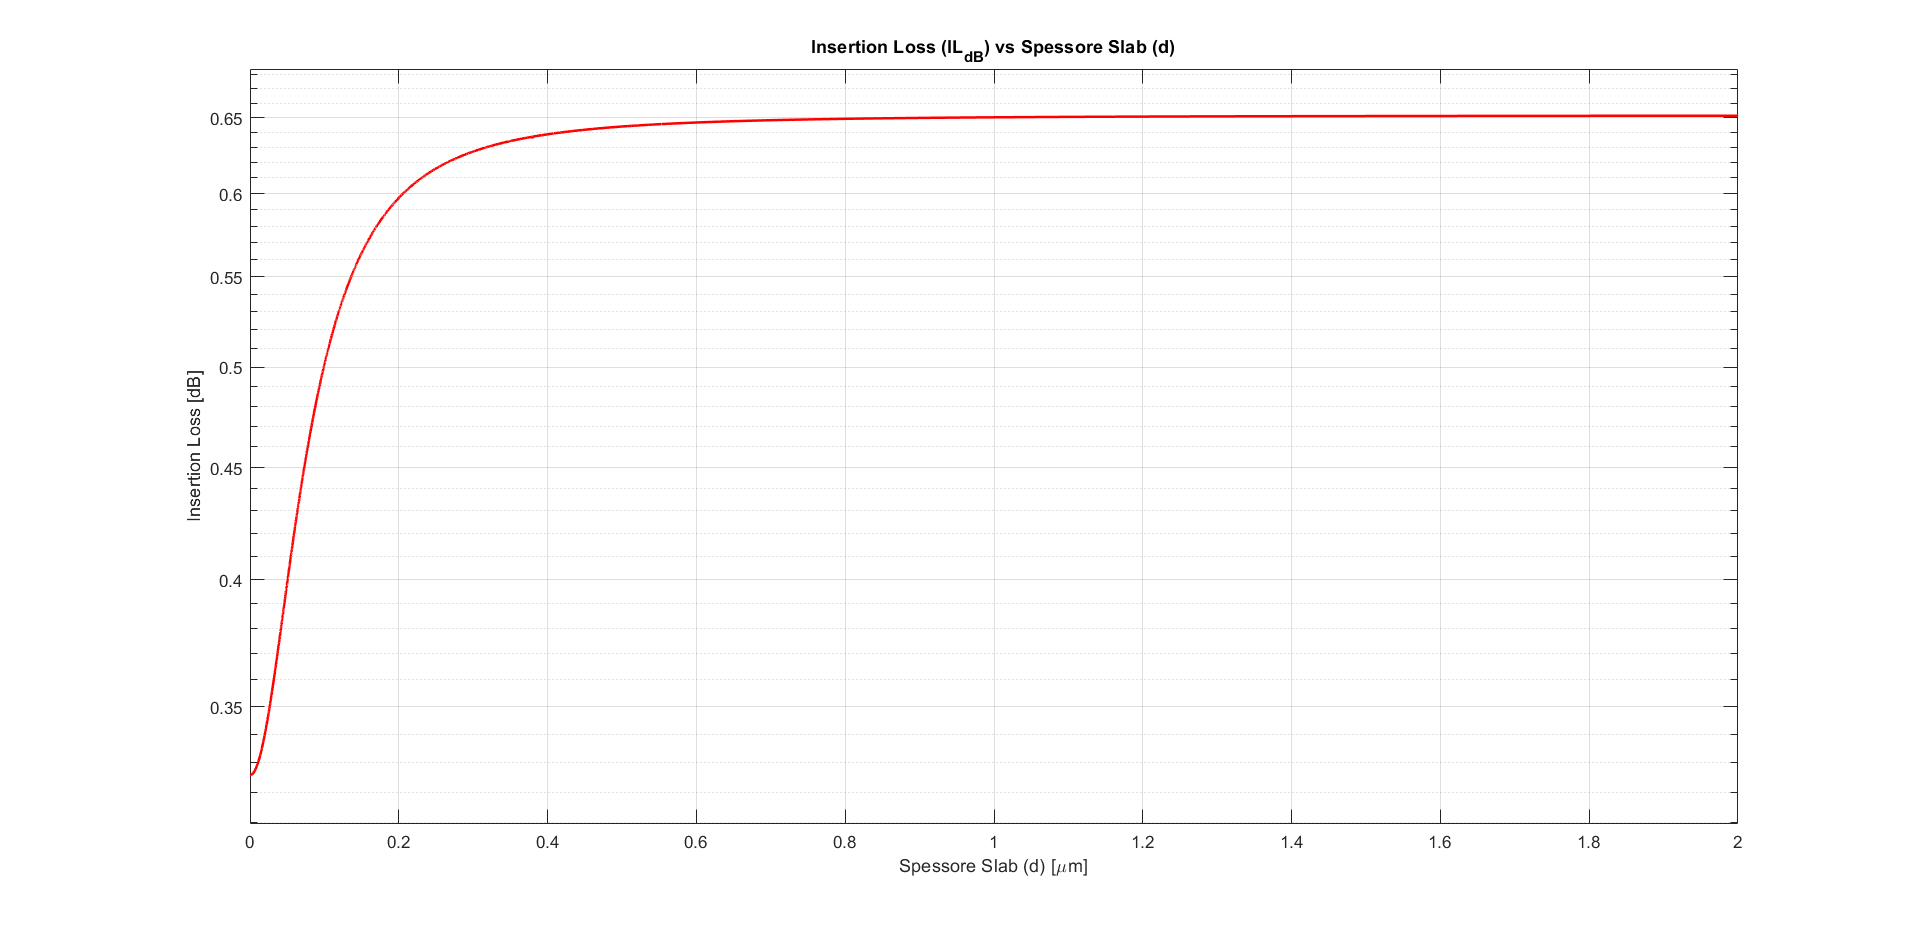
\includegraphics[width=15cm]{lab1/Images/prob1/IL_vs_d.png}
  \caption{Plot di $IL_{dB}$ in funzione di $d$ per il modo $TE_0$ , con $L = 5 \, mm$}
  \label{fig:IL_vs_d}
\end{figure}

\subsection{Scelta dello spessore $\boldsymbol{d_{SM}}$ per avere solo il modo $\boldsymbol{TE_0}$}

Si vuole scegliere un valore dello spessore $d$ tale da garantire la propagazione
del solo modo fondamentale $TE_0$, evitando la propagazione del primo modo
superiore $TE_1$.\\
\noindent\\ Inoltre, lo spessore scelto deve garantire un fattore di confinamento ottico
$\Gamma_{TE_0}$ compreso tra il $70\%$ e l'$80\%$. Il valore target scelto
per il calcolo è stato $\Gamma_{TE_0} = 0.75$. Questo parametro è cruciale per garantire
che il segnale rimanga principalmente confinato nel core, minimizzando le perdite nel cladding.\\
\noindent\\ Il valore dello spessore $d$ che soddisfa le condizioni sopra descritte è stato
denominato $\boldsymbol{d_{SM}}$ e risulta essere:
\[
 \boldsymbol{d_{SM} = 0.1573 \, \mu m}
\]

\noindent\\

\subsection{Calcolo di $\boldsymbol{n_{eff}(\omega)}$ e $\boldsymbol{n_{eff}(\lambda)}$} 

Per la guida a singolo modo ottenuta con lo spessore $d_{SM}$, è stato calcolato
l'indice di rifrazione efficace $n_{eff}$ per i modi $TE_0$ e $TE_1$ al variare
della pulsazione $\omega$ e della lunghezza d'onda $\lambda$.\\
\noindent\\ Il calcolo è stato effettuato per un intervallo di lunghezze d'onda
compreso tra $1100\,nm$ e $1620\,nm$, tipico delle comunicazioni ottiche, che corrisponde
a un intervallo di pulsazioni compreso tra $1.16 \cdot 10^{15} \, rad/s$ e $1.71 \cdot 10^{15} \, rad/s$.

\noindent\\ Gli andamenti di $n_{eff}(\omega)$ e $n_{eff}(\lambda)$ sono rappresentati
 nelle Figure \ref{fig:neff_vs_omega} e \ref{fig:neff_vs_lambda} rispettivamente.

 \newpage

\begin{figure}[!h]
 \centering
 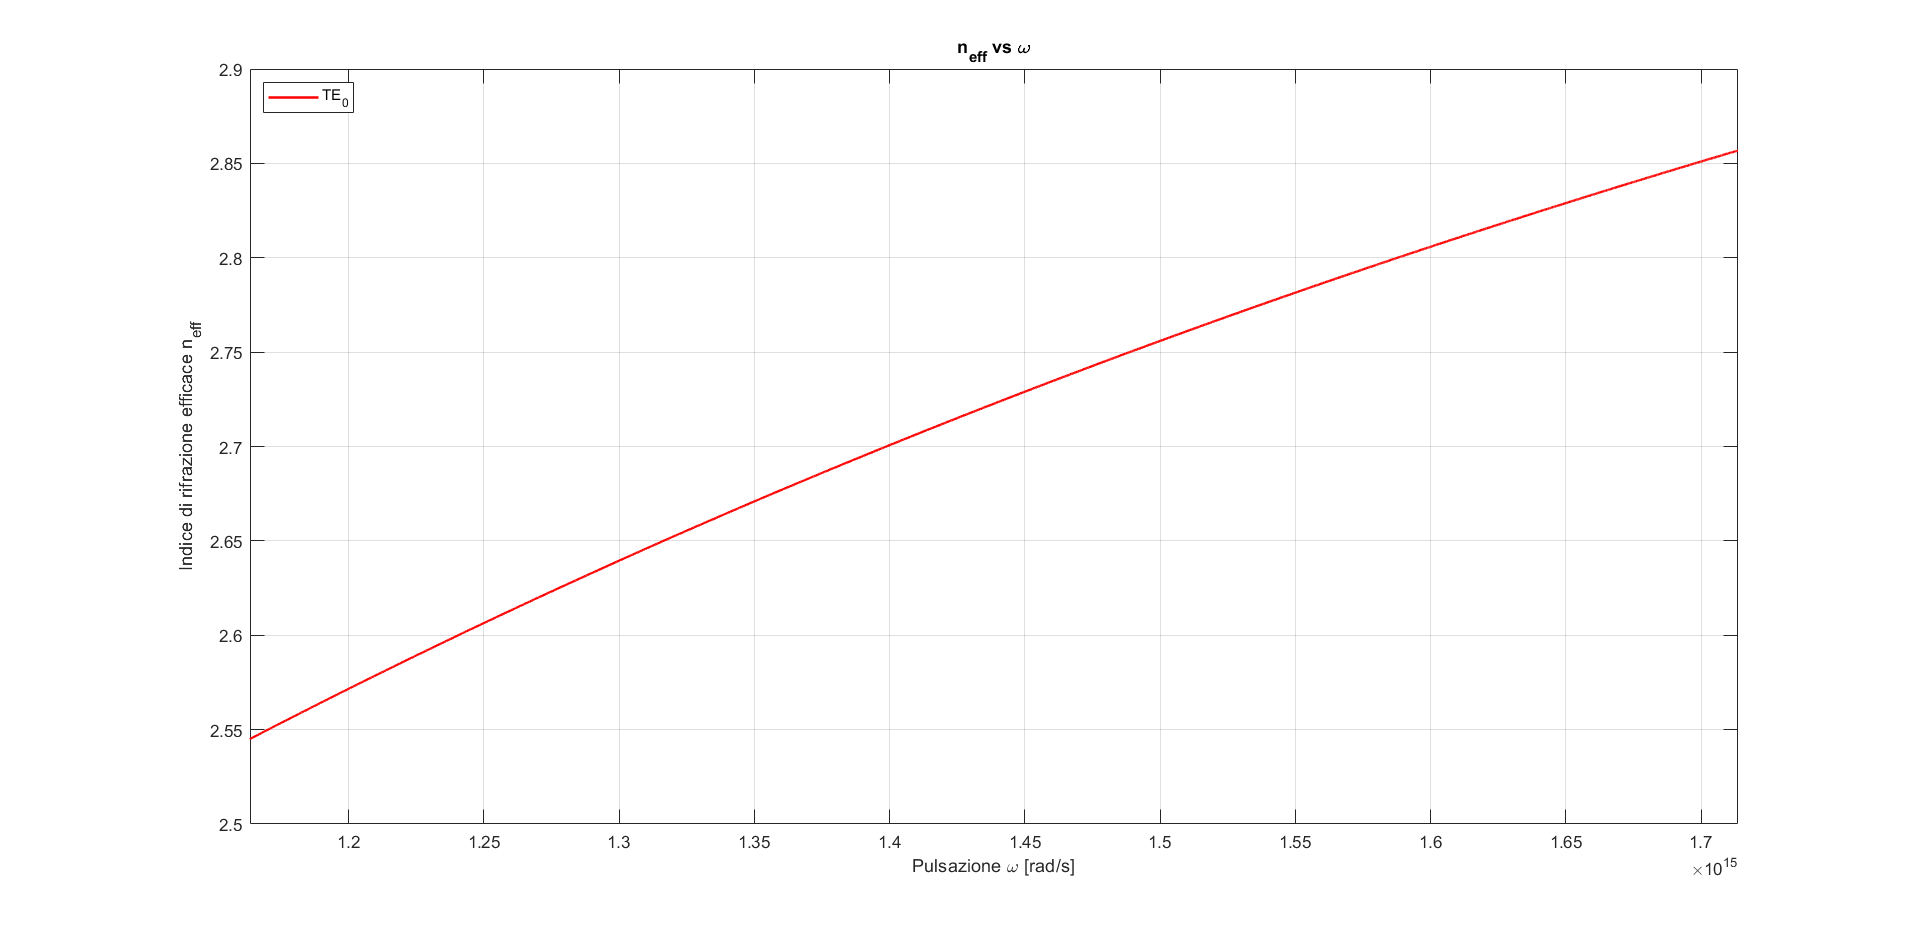
\includegraphics[width=15cm]{lab1/Images/prob1/neff_vs_omega.png}
  \caption{Plot di $n_{eff}$ in funzione di $\omega$ per il modo fondamentale $TE_0$}
  \label{fig:neff_vs_omega}
\end{figure}

\begin{figure}[!h]
 \centering
 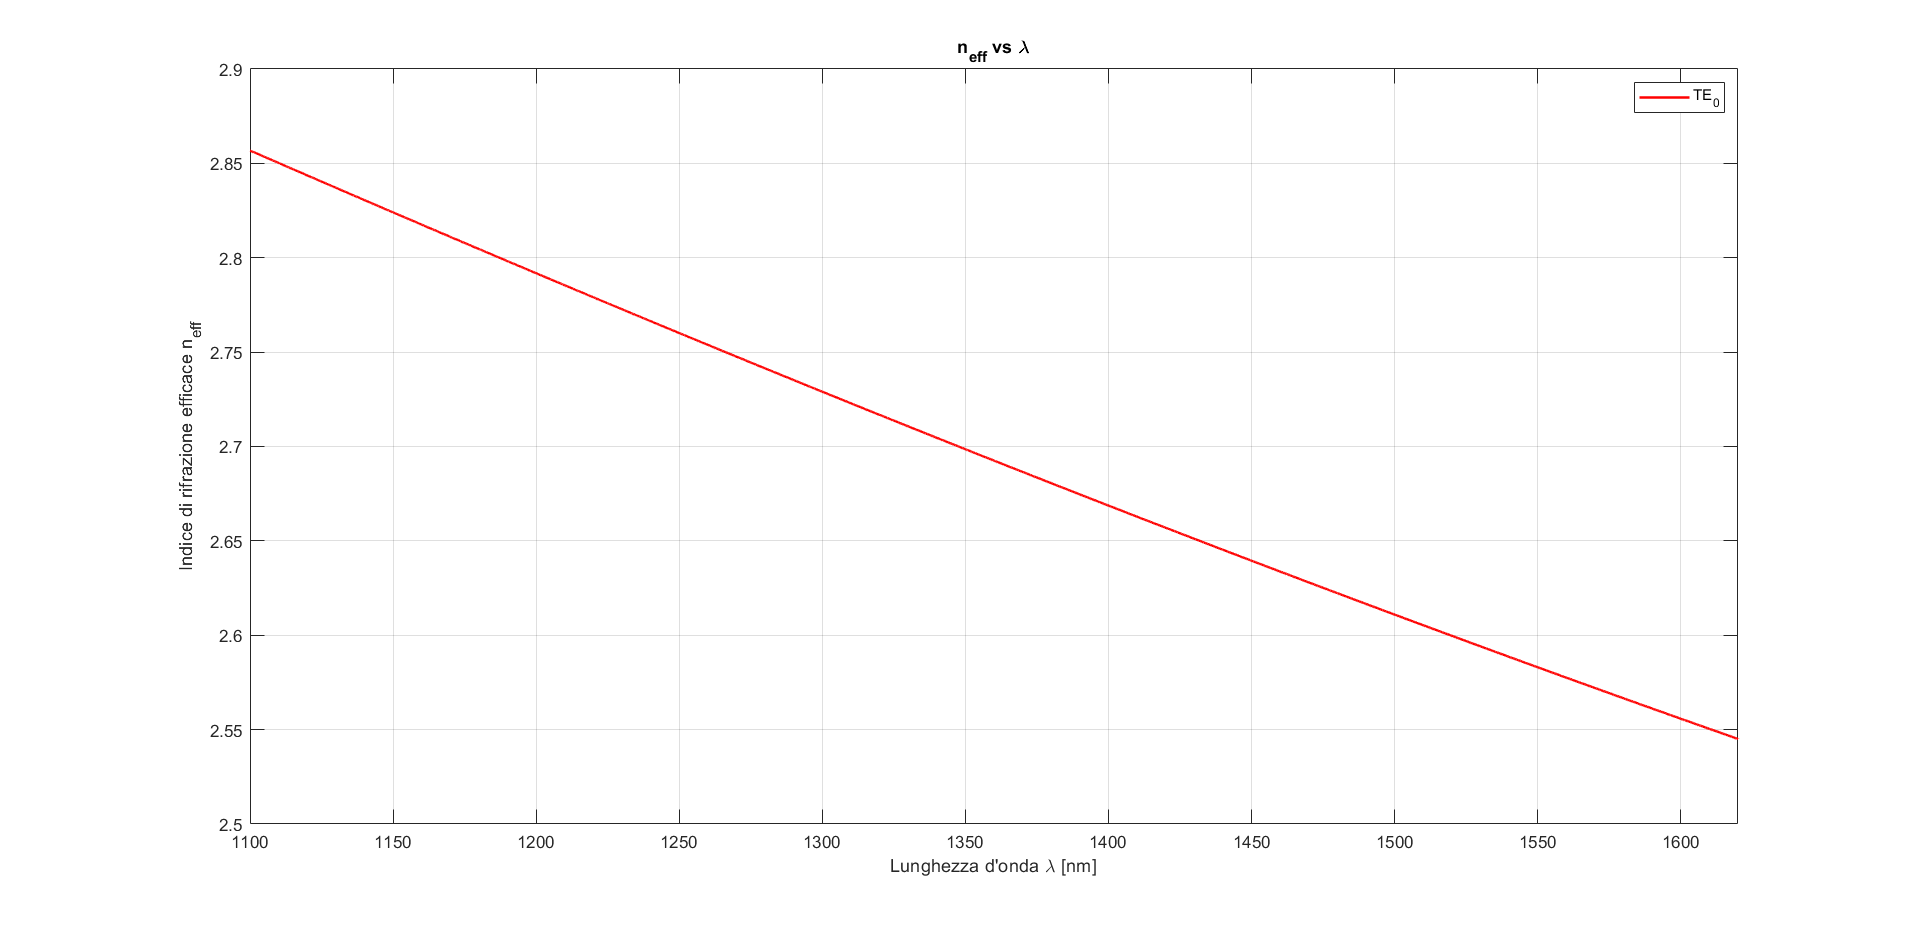
\includegraphics[width=15cm]{lab1/Images/prob1/neff_vs_lambda.png}
  \caption{Plot di $n_{eff}$ in funzione di $\lambda$ per il modo fondamentale $TE_0$}
  \label{fig:neff_vs_lambda}
\end{figure}

\noindent\\ Dai grafici riportati sopra si evince come l'indice di rifrazione efficace
per il modo $TE_0$ ($n_{eff,TE_0}$) aumenti al crescere della pulsazione $\omega$ e,
di conseguenza, diminuisca al crescere della lunghezza d'onda $\lambda$. In particolare,
i valori assunti da $n_{eff,TE_0}$ variano tra $2.54$ e $2.86$.
\noindent\\\\ Inoltre, ricordando che la guida è stata progettata per essere a singolo modo
(quindi con spessore del core pari a $d = d_{SM} = 0.1573 \, \mu m$), il modo $TE_1$ non si
propaga, quindi il suo indice di rifrazione efficace $n_{eff,TE_1}$ non è definito per la guida a singolo modo.\\
\\ Per questo motivo nei grafici precedenti è rappresentato soltanto l'andamento
di $n_{eff,TE_0}$, mentre $n_{eff,TE_1}$ non è riportato.\\

\newpage
\subsection{Calcolo e plot di $\boldsymbol{n_{g}(\omega)}$}
Infine, si è ricavato l'andamento dell'indice di rifrazione di gruppo $n_g$, al fine di analizzare
la dispersione cromatica. In particolare, l'indice di rifrazione di gruppo è legato alla velocità 
di gruppo $v_g$ attraverso la relazione:
\begin{equation}
    n_g = \frac{c}{v_g}
\end{equation}
 
\noindent dove $c$ è la velocità della luce nel vuoto. Pertanto, per calcolare $n_g$ è necessario prima calcolare
la velocità di gruppo $v_g$, che è definita come:
\begin{equation}
    v_g = \frac{\partial\omega}{\partial\beta} = \left(\frac{\partial\beta}{\partial\omega}\right)^{-1} = \frac{1}{\frac{1}{c} n_{eff} + \frac{\omega}{c}\frac{\partial n_{eff}}{\partial \omega}} = \frac{c}{n_{eff} + \omega\frac{\partial n_{eff}}{\partial \omega}}
\end{equation}

\noindent\\ Ne deriva che l'espressione dell'indice di rifrazione di gruppo è la seguente:
\begin{equation}
    n_g(\omega) = n_{eff}(\omega) + \omega\frac{\partial n_{eff}(\omega)}{\partial \omega}
\end{equation}

\noindent
\subsubsection*{Calcolo del termine $\boldsymbol{\dfrac{\partial n_{eff}(\omega)}{\partial \omega}}$}

\noindent Per calcolare $n_g(\omega)$ è quindi fondamentale calcolare il termine $\frac{\partial n_{eff}}{\partial \omega}$, che rappresenta la variazione dell'indice di rifrazione efficace al variare della pulsazione.\\
Per fare ciò, si riscrive l'equazione trascendente \ref{eq:d} riportata in precedenza (ponendo $m = 0$) come segue:
\[
    k_x \cdot d = tan^{-1}\left(\frac{\gamma}{k_x}\right) + tan^{-1}\left(\frac{\delta}{k_x}\right)
\]

\noindent e noto che $\gamma = \delta$, allora l'equazione trascendente diventa:
\[
    k_x \cdot d = 2 \cdot tan^{-1}\left(\frac{\gamma}{k_x}\right)
\]

\noindent\\ Il rapporto $\frac{\gamma}{k_x}$ può essere riscritto in funzione di $n_{eff}$ come: 
\[
\frac{\gamma}{k_x} = \frac{\sqrt{n_{eff}^2 - n_2^2}}{\sqrt{n_1^2 - n_{eff}^2}}
\]
\noindent quindi l'equazione complessiva risulta essere (sostituendo $n_{eff}$ con $n$ per una migliore leggibilità):

\[
    \frac{\omega \cdot d}{c} \sqrt{n_1^2 - n^2} - 2 \cdot tan^{-1}\left(\frac{\sqrt{n^2 - n_2^2}}{\sqrt{n_1^2 - n^2}}\right) = 0
\]

\noindent\\ Visto che $n = n_{eff}(\omega)$, si può derivare l'equazione precedente rispetto a $\omega$ per ottenere $\frac{\partial n_{eff}}{\partial \omega}$.\\
\\Ponendo $A = \sqrt{n_1^2 - n^2}$ e $B = \sqrt{n^2 - n_2^2}$ e derivando rispetto a $\omega$, l'equazione trascendente diventa:
\[
    \frac{\partial}{\partial \omega} \left[\frac{\omega \cdot d}{c} A\right] - 2 \frac{\partial}{\partial \omega} \left[tan^{-1}\left(\frac{B}{A}\right)\right] = 0
\]

\subsubsection*{Calcolo dei termini derivati}

\noindent Applicando la derivata al primo termine:
\[
    \frac{\partial}{\partial \omega} \left[\frac{\omega \cdot d}{c} A\right] = \frac{d}{c} A + \frac{\omega \cdot d}{c} \frac{\partial A}{\partial \omega}
\]
\noindent Cambiando differenziale, possiamo scrivere:
\[
    \frac{\partial A}{\partial \omega} = \frac{\partial A}{\partial n} \cdot \frac{\partial n}{\partial \omega} = \frac{1}{2\sqrt{n_1^2 - n^2}} \cdot (-2n) \cdot \frac{\partial n}{\partial \omega} =  -\frac{n}{A} \cdot \frac{\partial n}{\partial \omega}
\]
\noindent In definitiva, il primo termine diventa:
\[
    \frac{\partial}{\partial \omega} \left[\frac{\omega \cdot d}{c} A\right] = \frac{d}{c} A - \frac{\omega \cdot d}{c} \frac{n}{A} \cdot \frac{\partial n}{\partial \omega}
\]  

\newpage
\noindent Per quanto riguarda il secondo termine, si ricorda che la derivata dell'arcotangente risulta essere:
\[
    \frac{\partial}{\partial x} tan^{-1}(x) = \frac{1}{1+x^2}
\]
\noindent Quindi, applicando la derivata al secondo termine:
\[
    \frac{\partial}{\partial \omega} \left[tan^{-1}\left(\frac{B}{A}\right)\right] = \frac{1}{1 + \left(\frac{B}{A}\right)^2} \cdot \frac{\partial}{\partial \omega} \left(\frac{B}{A}\right)
\]
\noindent come fatto in precedenza, applicando un cambio del differenziale possiamo scrivere:
\[
    \frac{\partial}{\partial \omega} \left(\frac{B}{A}\right) = \frac{\partial}{\partial n} \left(\frac{B}{A}\right) \cdot \frac{\partial n}{\partial \omega}
\]
\noindent Applicando la derivata del quoziente, si ottiene:
\[
    \frac{\partial}{\partial n} \left(\frac{B}{A}\right) = \frac{A \cdot \frac{\partial B}{\partial n} - B \cdot \frac{\partial A}{\partial n}}{A^2}
\]

\noindent L'espressione finale, dopo varie semplificazioni algebriche, risulta essere:
\[
    \frac{\partial}{\partial \omega} \left[tan^{-1}\left(\frac{B}{A}\right)\right] = \frac{n}{A \cdot B} \frac{\partial n}{\partial \omega}
\]

\noindent\\ Come risultato finale, possiamo scrivere l'intera equazione trascendente come segue:
\[
    \frac{d}{c} A - \frac{\omega \cdot d}{c} \frac{n}{A} \cdot \frac{\partial n}{\partial \omega} - 2 \cdot \frac{n}{A \cdot B} \frac{\partial n}{\partial \omega} = 0
\]

\noindent\\ Infine, isolando $\frac{\partial n}{\partial \omega}$ e sostituendo le espressioni di $A$, $B$ e $n$, otteniamo:
\begin{equation}
    \dfrac{\partial n_{eff}(\omega)}{\partial \omega} = \dfrac{\dfrac{d}{c} \sqrt{n_1^2 - n_{eff}^2(\omega)}}{\dfrac{\omega \cdot d}{c} \dfrac{n_{eff}(\omega)}{\sqrt{n_1^2 - n_{eff}^2(\omega)}} + 2 \cdot \dfrac{n_{eff}(\omega)}{\sqrt{n_1^2 - n_{eff}^2(\omega)} \cdot \sqrt{n_{eff}^2(\omega) - n_2^2}}}
\end{equation}

\noindent\\\\ A questo punto, sostituendo il termine $\frac{\partial n_{eff}(\omega)}{\partial \omega}$ nell'espressione di $n_g(\omega)$, si ottiene l'andamento dell'indice di rifrazione di gruppo in funzione della pulsazione $\omega$, riportato in Figura \ref{fig:ng_vs_omega}.\\

\begin{figure}[!h]
 \centering
 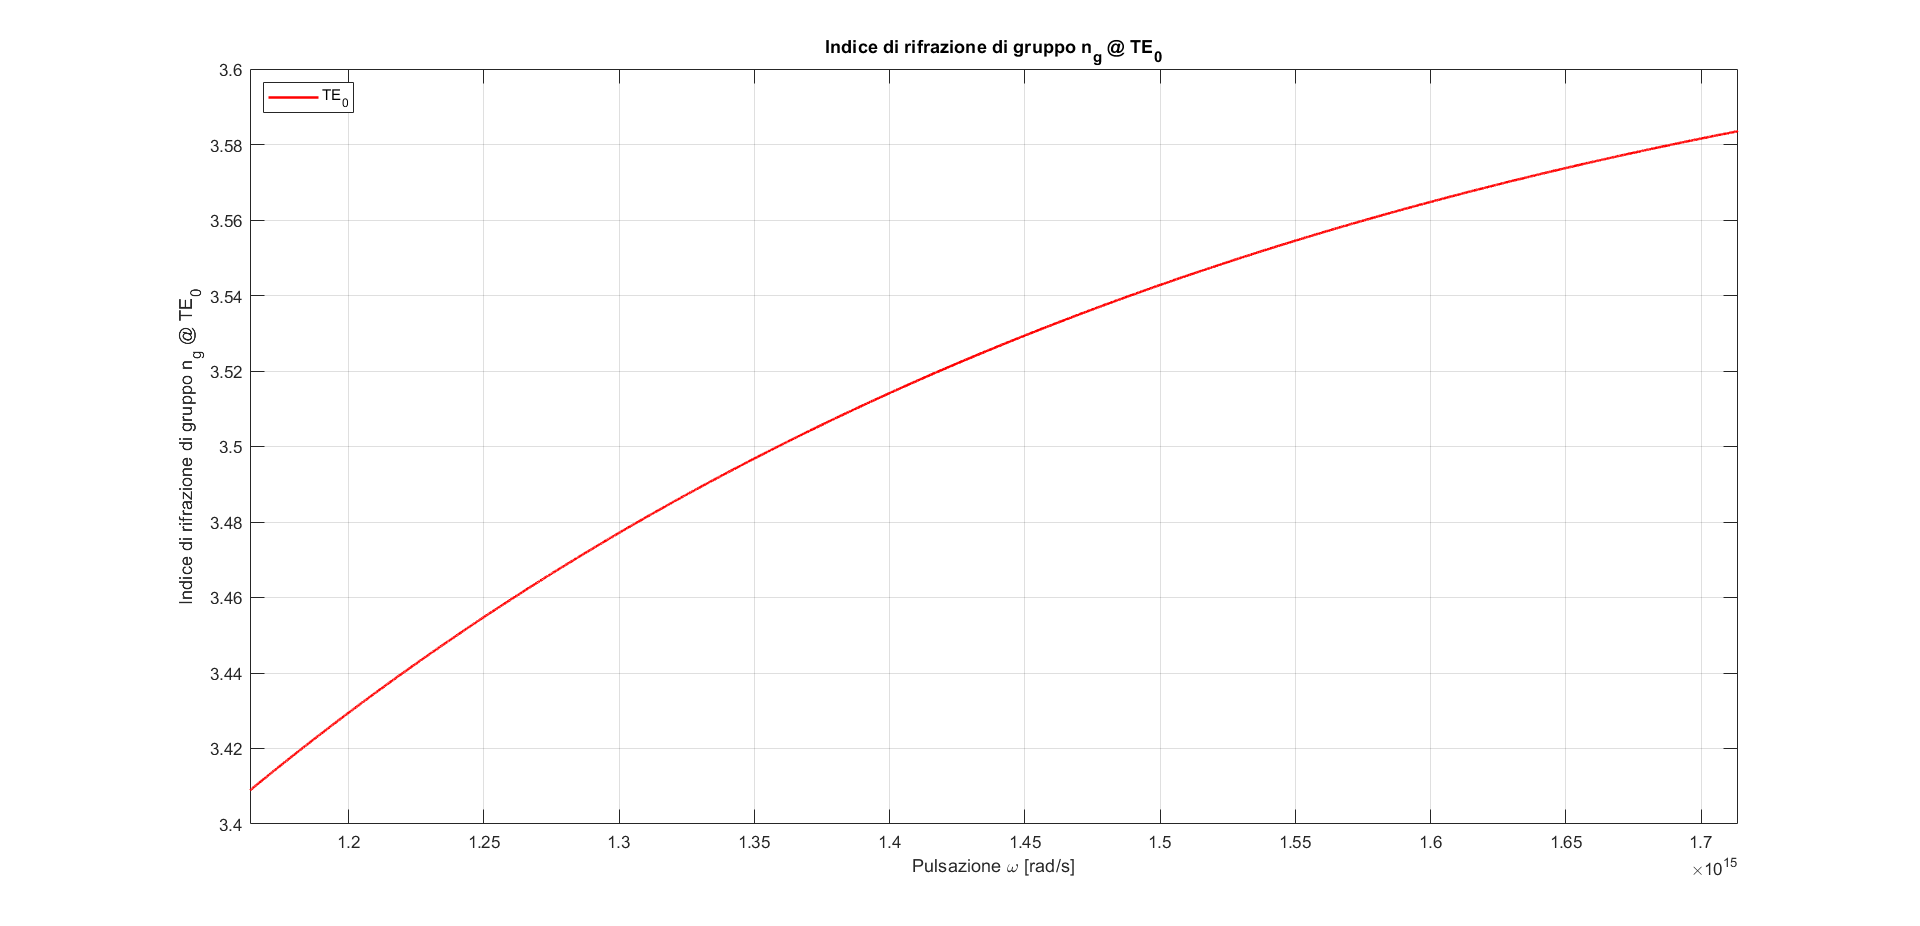
\includegraphics[width=15cm]{lab1/Images/prob1/ng_vs_omega.png}
  \caption{Plot dell'indice di rifrazione di gruppo $n_{g}(\omega)$ in funzione di $\omega$ }
  \label{fig:ng_vs_omega}
\end{figure}


%%%%%%   Secondo esercizio --------------------------------------
\newpage
\section{Propagazione di impulsi ottici in fibra ottica dispersiva}
L'obiettivo del secondo Assignment del Laboratorio 1 è lo studio della propagazione di impulsi ottici in una fibra ottica dispersiva, approfondendo l'impatto della dispersione cromatica.

\subsection{Definizione dell'impulso}
L'impulso in analisi può essere considerato come un modello molto semplificato, che rappresenti una specifica sequenza di bit, ossia "010". Di conseguenza, l'impulso ottico può essere rappresentato
come una funzione super-gaussiana, definita come segue:
\begin{equation}
    p(t) = e^{-\left(\dfrac{t}{\tau_{0}}\right)^4}
\end{equation}

\noindent In particolare, sono stati considerati quattro impulsi ottici con durate caratteristiche differenti, ossia $\tau_{0} = 0.5 \, ns$, $\tau_{0} = 0.1 \, ns$, $\tau_{0} = 10 \, ps$ e $\tau_{0} = 5 \, ps$, per analizzare l'effetto della dispersione cromatica su impulsi di diversa durata.\\

\subsection{Plot degli impulsi e misura del FWHM}
\noindent Gli impulsi ottici definiti in precedenza sono stati plottati in funzione del tempo, come mostrato in Figura \ref{fig:pin_t}.

\begin{figure}[!h]
 \centering
 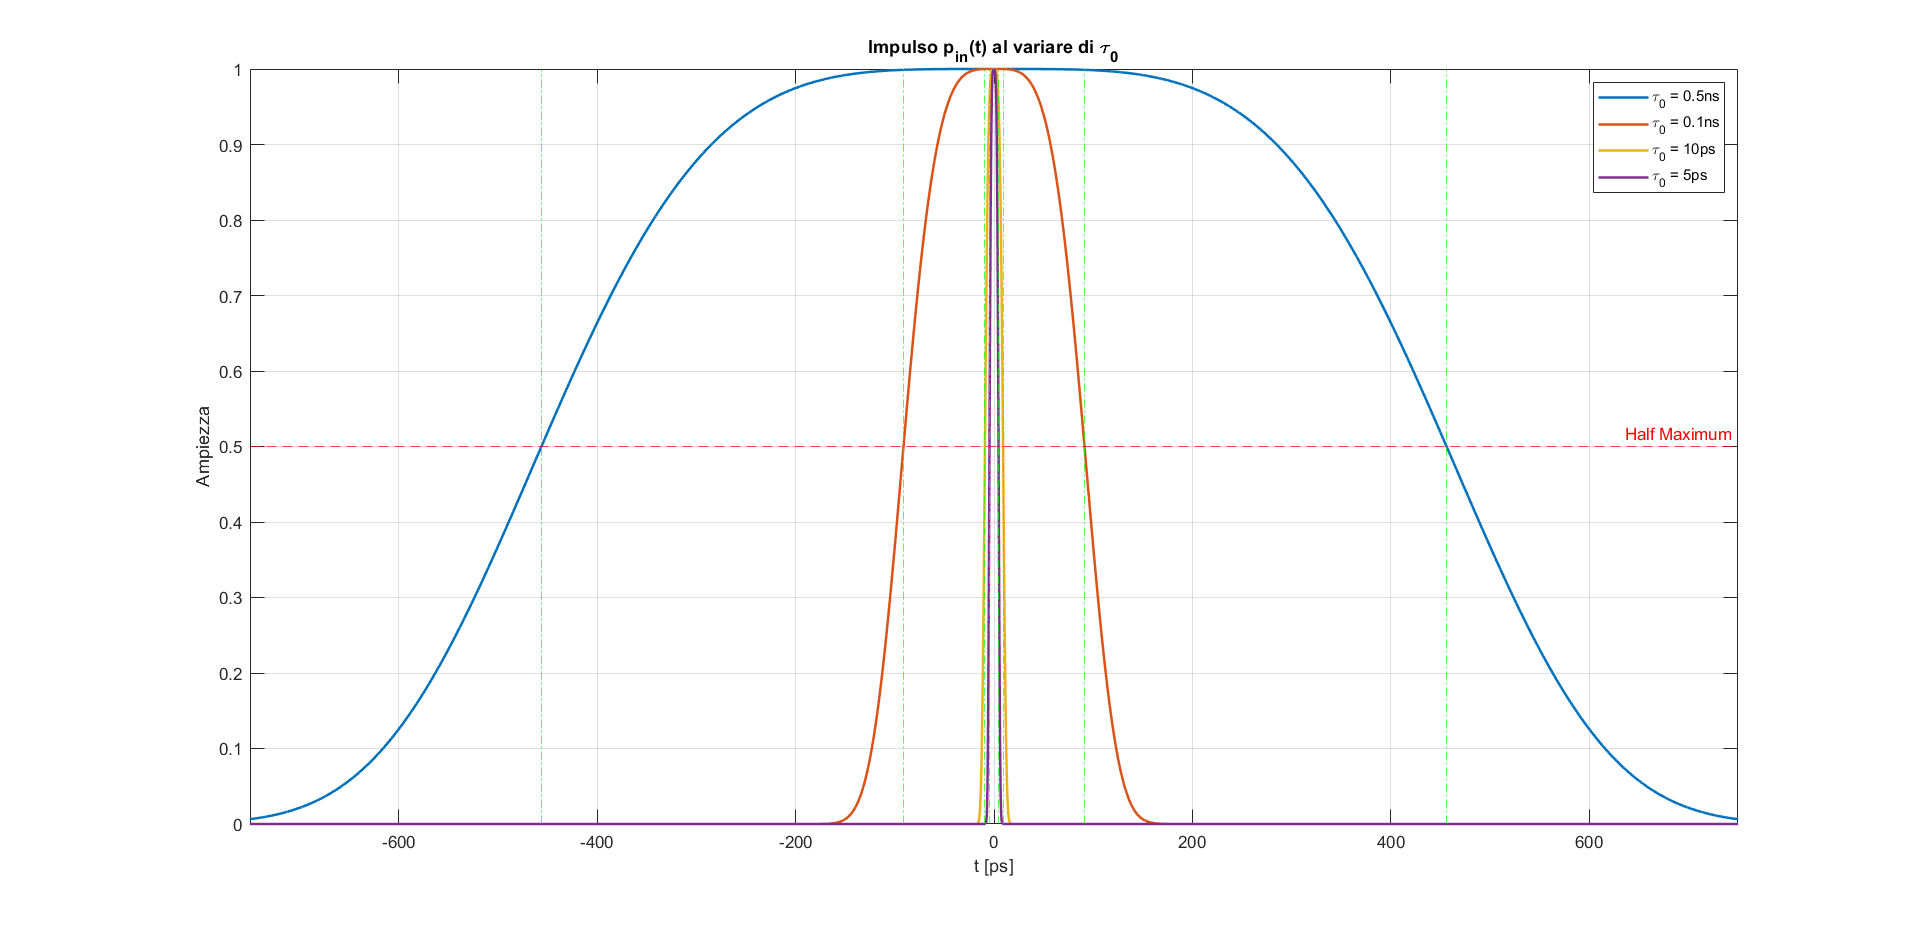
\includegraphics[width=15cm]{lab1/Images/prob2/pin_t.png}
  \caption{Plot degli impulsi ottici $p_{in}(t)$ in funzione del tempo}
  \label{fig:pin_t}
\end{figure}

\noindent Inoltre, per ciascun impulso è stato calcolato il valore del FWHM (Full Width at Half Maximum), ossia la larghezza dell'impulso a metà altezza, che rappresenta una misura della durata dell'impulso stesso. I valori del FWHM per ciascun impulso sono riportati in Tabella \ref{tab:FWHM}.  

\begin{table}[!h]
    \centering
    \begin{tabular}{|c|c|}
    \hline
    \textbf{Durata $\boldsymbol{\tau_{0}}$} & \textbf{FWHM} \\ \hline \hline
    $0.5\,ns$           & $0.9124\,ns$  \\ \hline
    $0.1\,ns$           & $0.1824\,ns$  \\ \hline
    $10\,ps$            & $18.24\,ps$   \\ \hline
    $5\,ps$             & $9.12\,ps$    \\ \hline
    \end{tabular}
    \caption{Valori del FWHM per ciascun impulso ottico}
    \label{tab:FWHM}
\end{table}

\noindent Come facilmente prevedibile, ad una costante di tempo più piccola corrisponde un impulso più stretto e, di conseguenza, una minore FWHM.

\subsection{Calcolo e plot dello spettro ottico}
Per calcolare l'impulso in uscita si passa al dominio della frequenza, calcolando così lo spettro del segnale ottico. Il passaggio dal dominio del tempo a quello della frequenza
è effettuato tramite la trasformata di Fourier ed è di fondamentale importanza, dato che ogni componente spettrale $\omega$ dell'impulso subisce una rotazione di fase data da
$e^{-j\beta(\omega)z}$. Inoltre, visto che la fibra ottica in esame è dispersiva, si ha che $\beta(\omega)$ non è funzione lineare di $\omega$. Nella Figura \ref{fig:pin_f} è riportato
lo spettro ottico degli impulsi ottici definiti in precedenza, calcolato mediante le funzioni MATLAB \texttt{fft} e \texttt{fftshift}.

\begin{figure}[!h]
 \centering
 \includegraphics[width=15cm]{lab1/Images/prob2/pin_f.png}
  \caption{Plot degli spettri ottici $P_{in}(f)$ al variare di $\tau_0$ in funzione della frequenza}
  \label{fig:pin_f}
\end{figure}

\noindent Dalla Figura riportata sopra, si nota come all'aumentare di $\tau_0$ corrisponda una "compressione" nel dominio della frequenza; ciò significa che i segnali con una
costante di tempo maggiore varino più lentamente e quindi abbiano meno componenti ad alta frequenza.
\noindent\\

\subsection{Calcolo e plot della costante di propagazione $\boldsymbol{\beta(\omega)}$}

La costante di propagazione $\beta(\omega)$ può essere approssimata nella banda di interesse, calcolandone lo sviluppo in serie di Taylor.
\noindent\\\\ In particolare, data la lunghezza d'onda centrale $\lambda_0 = 1625 \, nm$, corrispondente a una pulsazione $\omega_0 = 2\pi \frac{c}{\lambda_0} \approx 1.16 \cdot 10^{15} \, rad/s$,
si è calcolato lo sviluppo in serie di Taylor nell'intorno della pulsazione centrale $\omega_0$, considerando i primi tre termini della serie.\\
\noindent\\ In questo modo, si ottiene l'espressione della costante di propagazione $\beta(\omega)$ in funzione della pulsazione $\omega$:
\begin{equation}
    \beta(\omega) = \beta_0 + \beta_1 (\omega - \omega_0) + \frac{1}{2} \beta_2 (\omega - \omega_0)^2
\end{equation}

\noindent dove
\[ 
\beta_0 = \beta(\omega_0), \quad \beta_1 = \left. \frac{\partial \beta}{\partial \omega} \right|_{\omega_0}, \quad \beta_2 = \left. \frac{\partial^2 \beta}{\partial \omega^2} \right|_{\omega_0}
\]
\noindent\\ sono rispettivamente la costante di propagazione, l'inverso della velocità di gruppo e un termine legato alla GVD (Group Velocity Dispersion), calcolate alla pulsazione centrale $\omega_0$.\\
\noindent\\ Si è quindi proceduto a plottare l'andamento di $\beta(\omega)$ in un range di $100 \, nm$ attorno a $\lambda_0$, come mostrato in Figura \ref{fig:beta_omega}.

\newpage
\begin{figure}[!h]
 \centering
 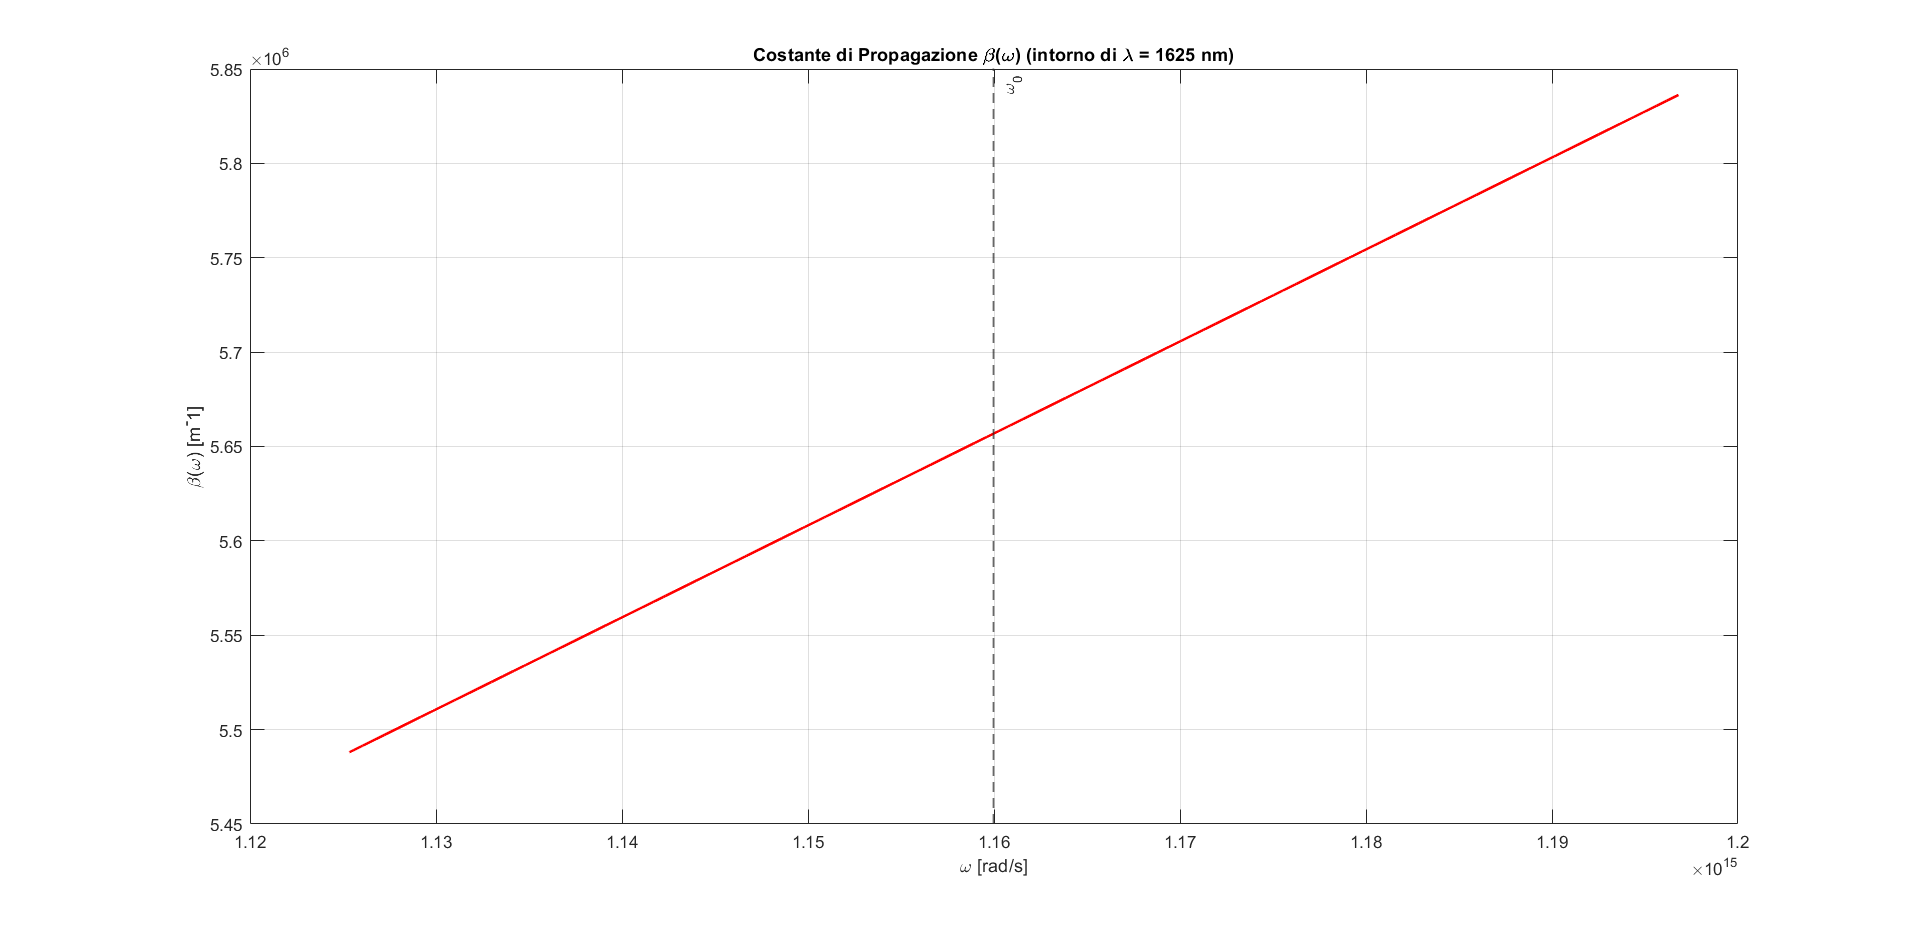
\includegraphics[width=13cm]{lab1/Images/prob2/beta_omega_int.png}
  \caption{Plot della costante di propagazione $\beta(\omega)$ in un range di $100 \, nm$ attorno a $\lambda_0$}
  \label{fig:beta_omega}
\end{figure}

\subsection{Calcolo e plot degli impulsi in uscita dalla fibra}
Successivamente, si è calcolata l'espressione degli impulsi in uscita dalla fibra ottica:
\begin{equation}
    P_{out}(\omega) = P_{in}(\omega) \cdot e^{-j\beta(\omega)L} e^{-(\alpha/2)\cdot L}
\end{equation}

\noindent considerando quattro lunghezze della fibra ottica, ossia $L = 1 \, m$, $L = 10 \, m$, $L = 1 \, km$ e $L = 80 \, km$.\\
\noindent Gli spettri d'uscita, con $\tau_0 = 0.5 \, ns$ e $\tau_0 = 5 \, ps$, sono riportati nelle Figure \ref{fig:pout_f_05ns} e \ref{fig:pout_f_5ps}.

\begin{figure}[!h]
 \centering
 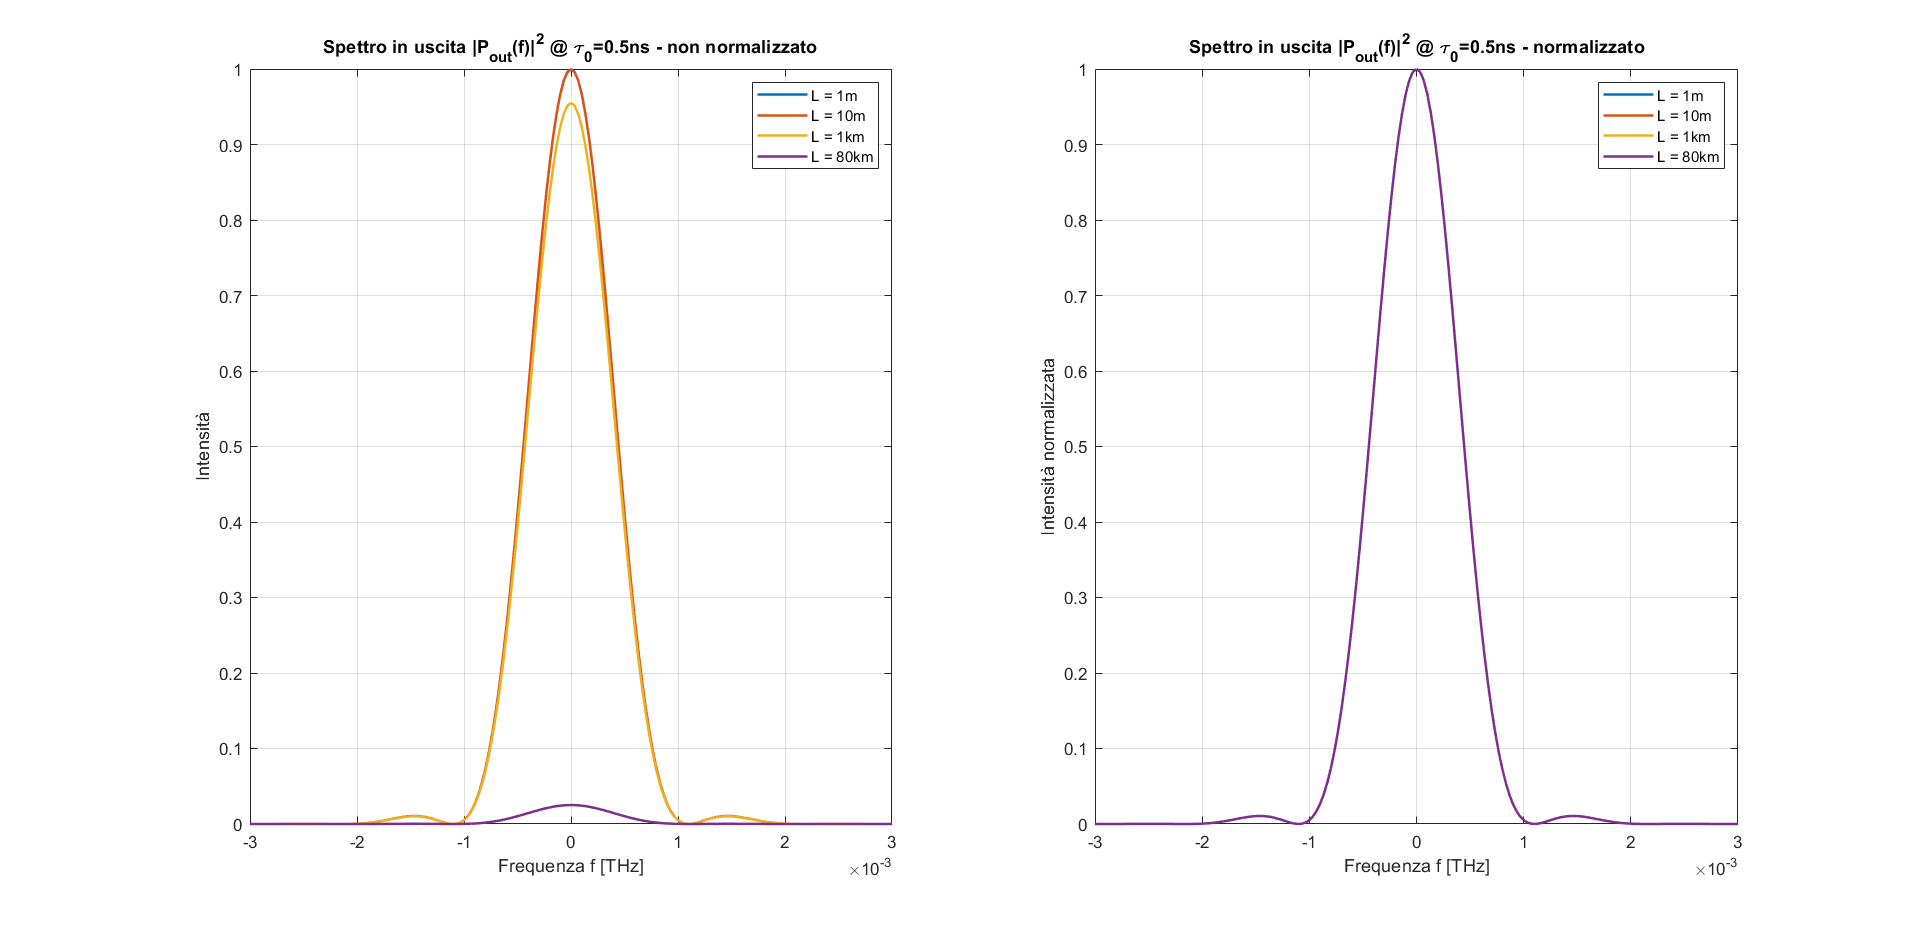
\includegraphics[width=15cm]{lab1/Images/prob2/Pout_f_05ns.png}
  \caption{Spettro dell'impulso in uscita dalla fibra $P_{out}(f)$ con $\tau_0 = 0.5 \, ns$}
  \label{fig:pout_f_05ns}
\end{figure}

\noindent In particolare, nella Figura \ref{fig:pout_f_05ns} si nota come l'impulso in uscita dalla fibra ottica non subisca alcuna distorsione,
considerando qualsiasi lunghezza possibile. Al fine di mettere in evidenza come il contenuto spettrale sia invariato, sono riportati sulla
parte destra dell'immagine gli impulsi con ampiezza normalizzata: risulta evidente che questi siano perfettamente sovrapposti.\\ 
Questo comportamento è perfettamente in linea con quanto previsto dalla teoria, in quanto il modulo dell'impulso in uscita può essere calcolato come:
\begin{equation}
    |P_{out}(\omega)| = |P_{in}(\omega)| \cdot |e^{-j\beta(\omega)L}| \cdot e^{-(\alpha/2)\cdot L} = |P_{in}(\omega)| \cdot e^{-(\alpha/2)\cdot L}
\end{equation}

\noindent Di conseguenza, normalizzando l'ampiezza degli impulsi, il termine di attenuazione non ha alcun effetto e quindi si ottengono delle forme d'onda identiche.  
\noindent Per poter apprezzare gli effetti della dispersione cromatica, che si manifesta nel dominio della frequenza come una variazione di fase, è necessario
considerare nuovamente gli impulsi nel dominio del tempo. In particolare, i principali effetti nel dominio del tempo causati dalla dispersione sono il \textit{broadening}
e la \textit{distorsione}.

\begin{figure}[!h]
 \centering
 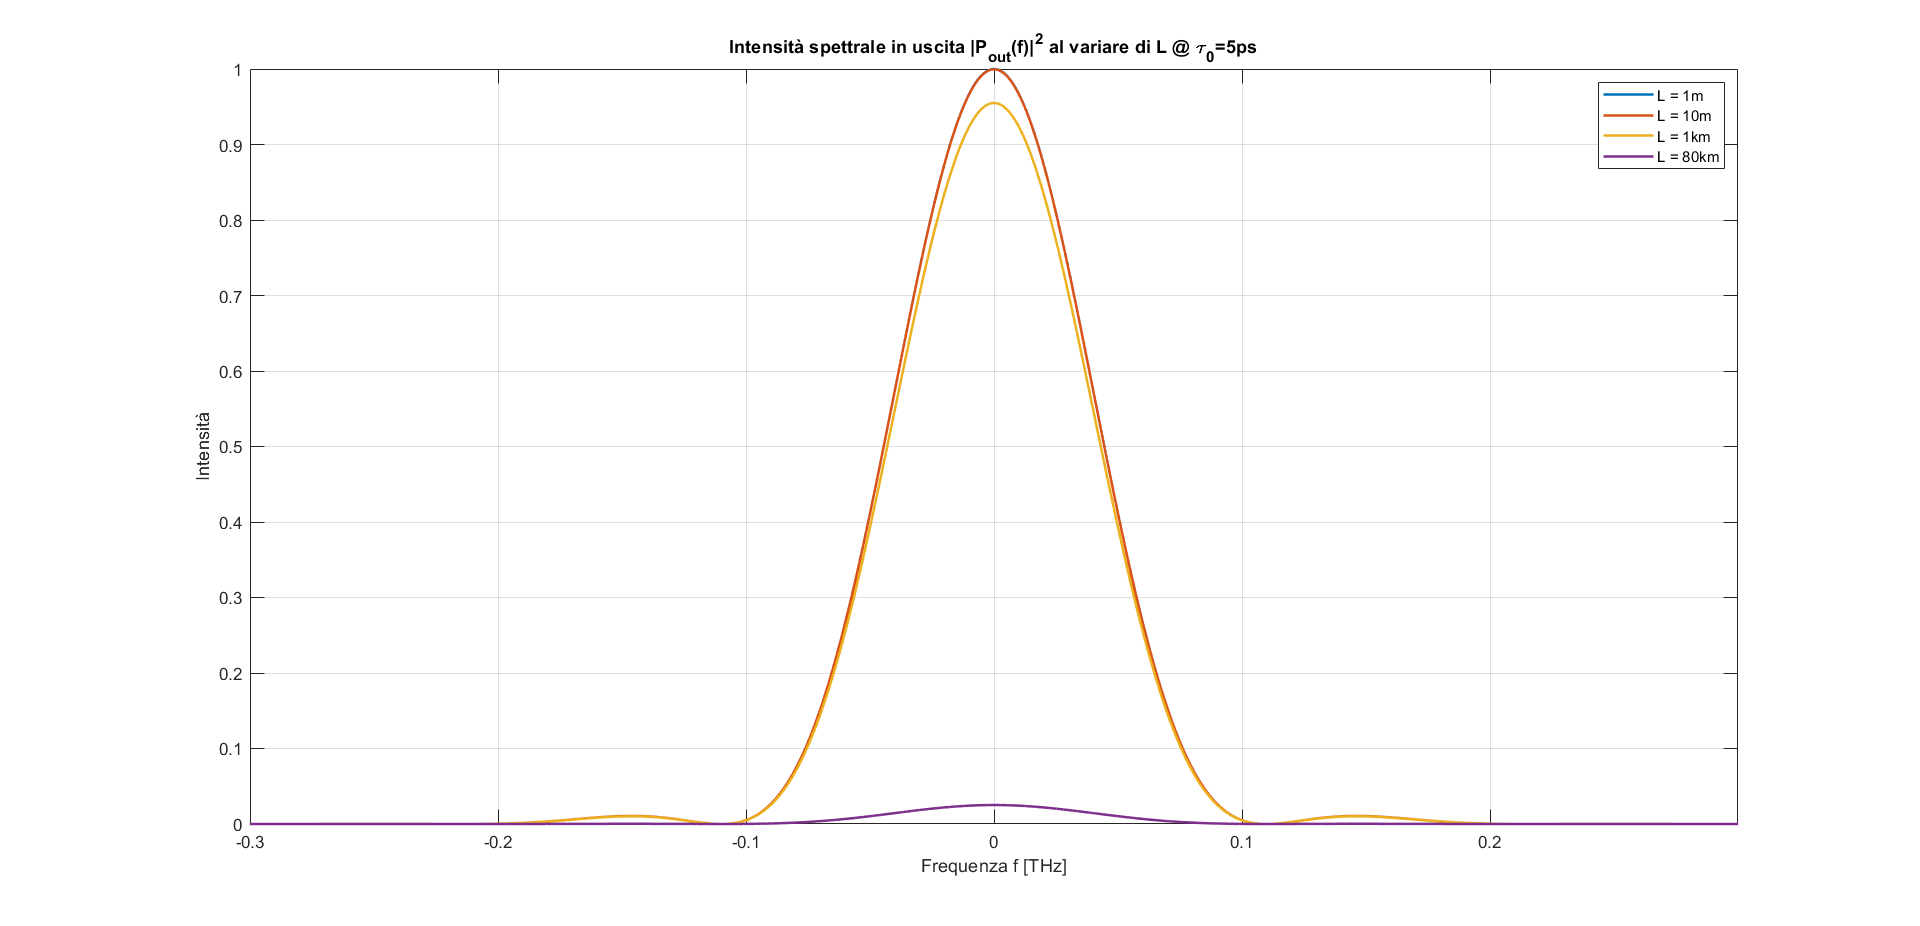
\includegraphics[width=12cm]{lab1/Images/prob2/Pout_f_5ps.png}
  \caption{Spettro dell'impulso in uscita dalla fibra $P_{out}(f)$ con $\tau_0 = 5 \, ps$}
  \label{fig:pout_f_5ps}
\end{figure}

\noindent Si è quindi proceduto a calcolare gli impulsi in uscita dalla fibra ottica nel dominio del tempo, sfruttando le funzioni MATLAB \texttt{ifft} e \texttt{ifftshift}.
Gli andamenti ottenuti sono riportati nelle Figure \ref{fig:pout_t_05ns} e \ref{fig:pout_t_5ps}.\\

\begin{figure}[!h]
 \centering
 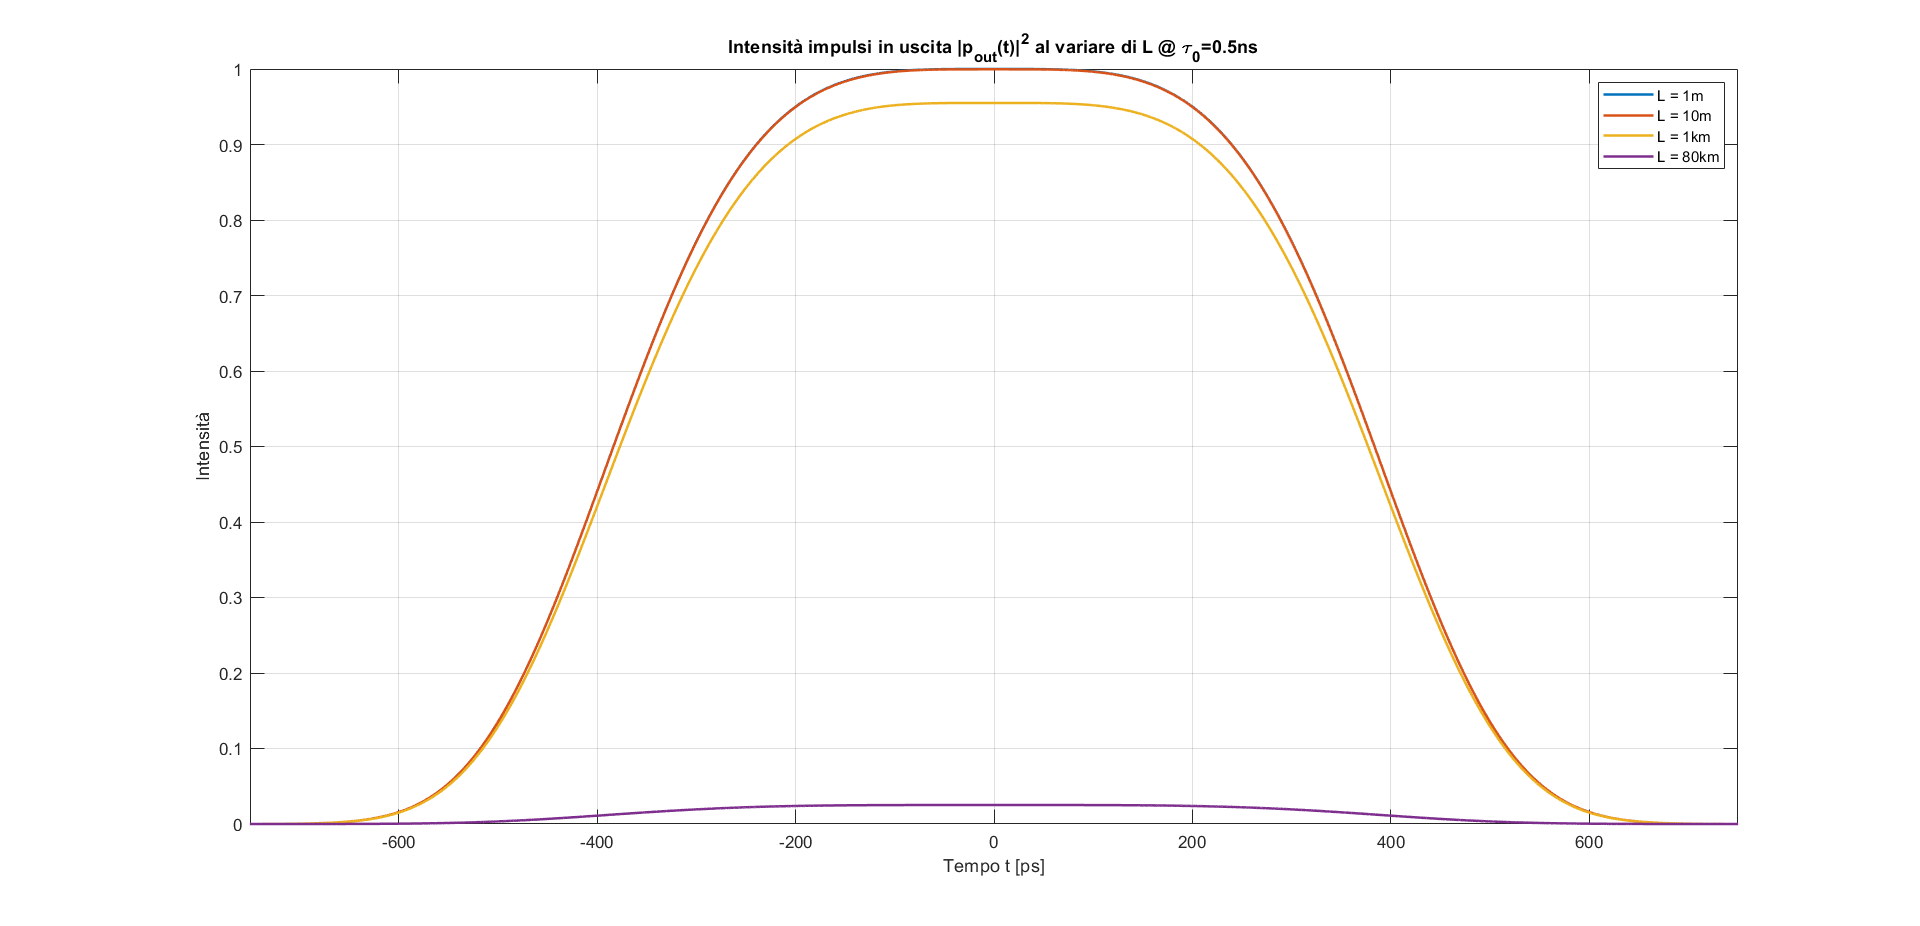
\includegraphics[width=14cm]{lab1/Images/prob2/pout_t_05ns.png}
  \caption{Impulso in uscita dalla fibra $p_{out}(t)$ con $\tau_0 = 0.5 \, ns$}
  \label{fig:pout_t_05ns}
\end{figure}

\begin{figure}[!h]
 \centering
 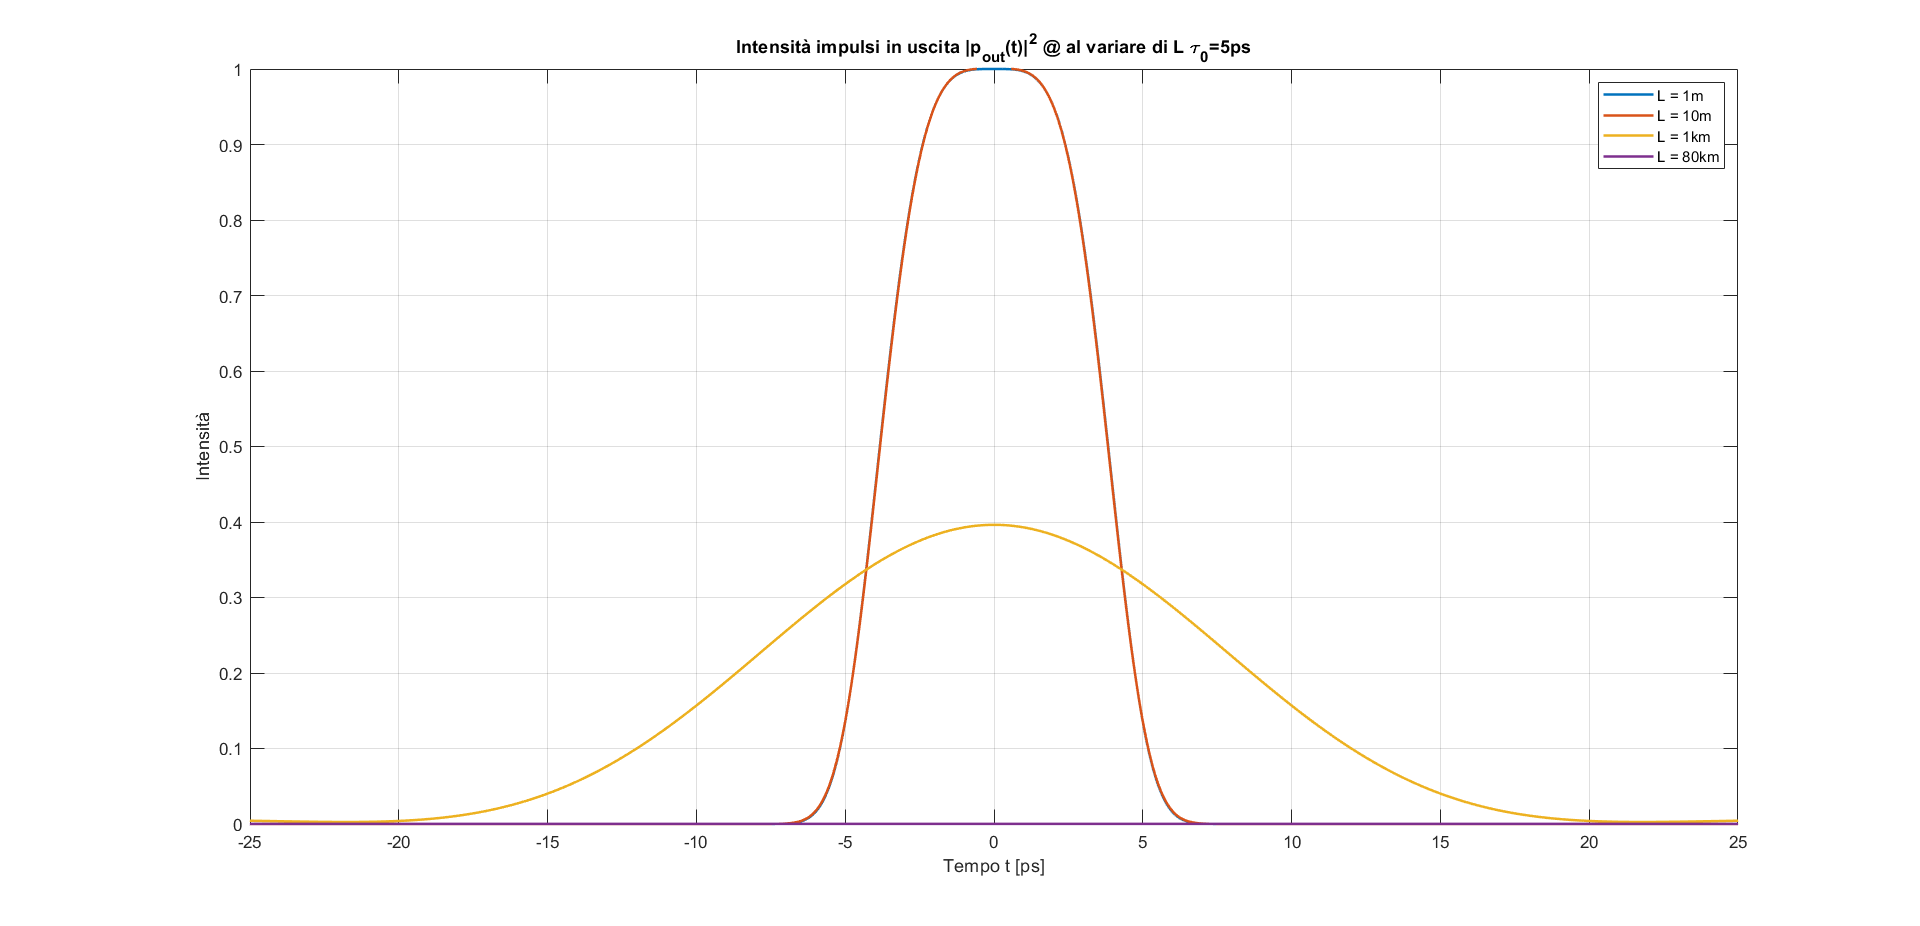
\includegraphics[width=14cm]{lab1/Images/prob2/pout_t_5ps.png}
  \caption{Impulso in uscita dalla fibra $p_{out}(t)$ con $\tau_0 = 5 \, ps$}
  \label{fig:pout_t_5ps}
\end{figure}

\subsection{Calcolo e plot di FWHM in uscita}
\noindent Sebbene le Figure \ref{fig:pout_t_05ns} e \ref{fig:pout_t_5ps} mostrino chiaramente l'effetto della dispersione cromatica,
che si manifesta principalmente sotto forma di broadening, ossia "allargamento" dell'impulso, è importante quantificare questi effetti.
\noindent\\\\ A tal proposito, per ciascun impulso ottico in uscita dalla fibra ottica, è stato calcolato il valore del FWHM: facendo un confronto con i valori del FWHM in ingresso,
è possibile quantificare l'effetto della dispersione cromatica sulla durata dell'impulso ottico.
\noindent\\\\ In Figura \ref{fig:FWHM_ratio} sono riportati i valori del rapporto tra il FWHM in uscita dalla fibra ottica e il FWHM in ingresso, in funzione della lunghezza della fibra e al variare
della durata caratteristica $\tau_0$ dell'impulso ottico in ingresso.

\begin{figure}[!h]
 \centering
 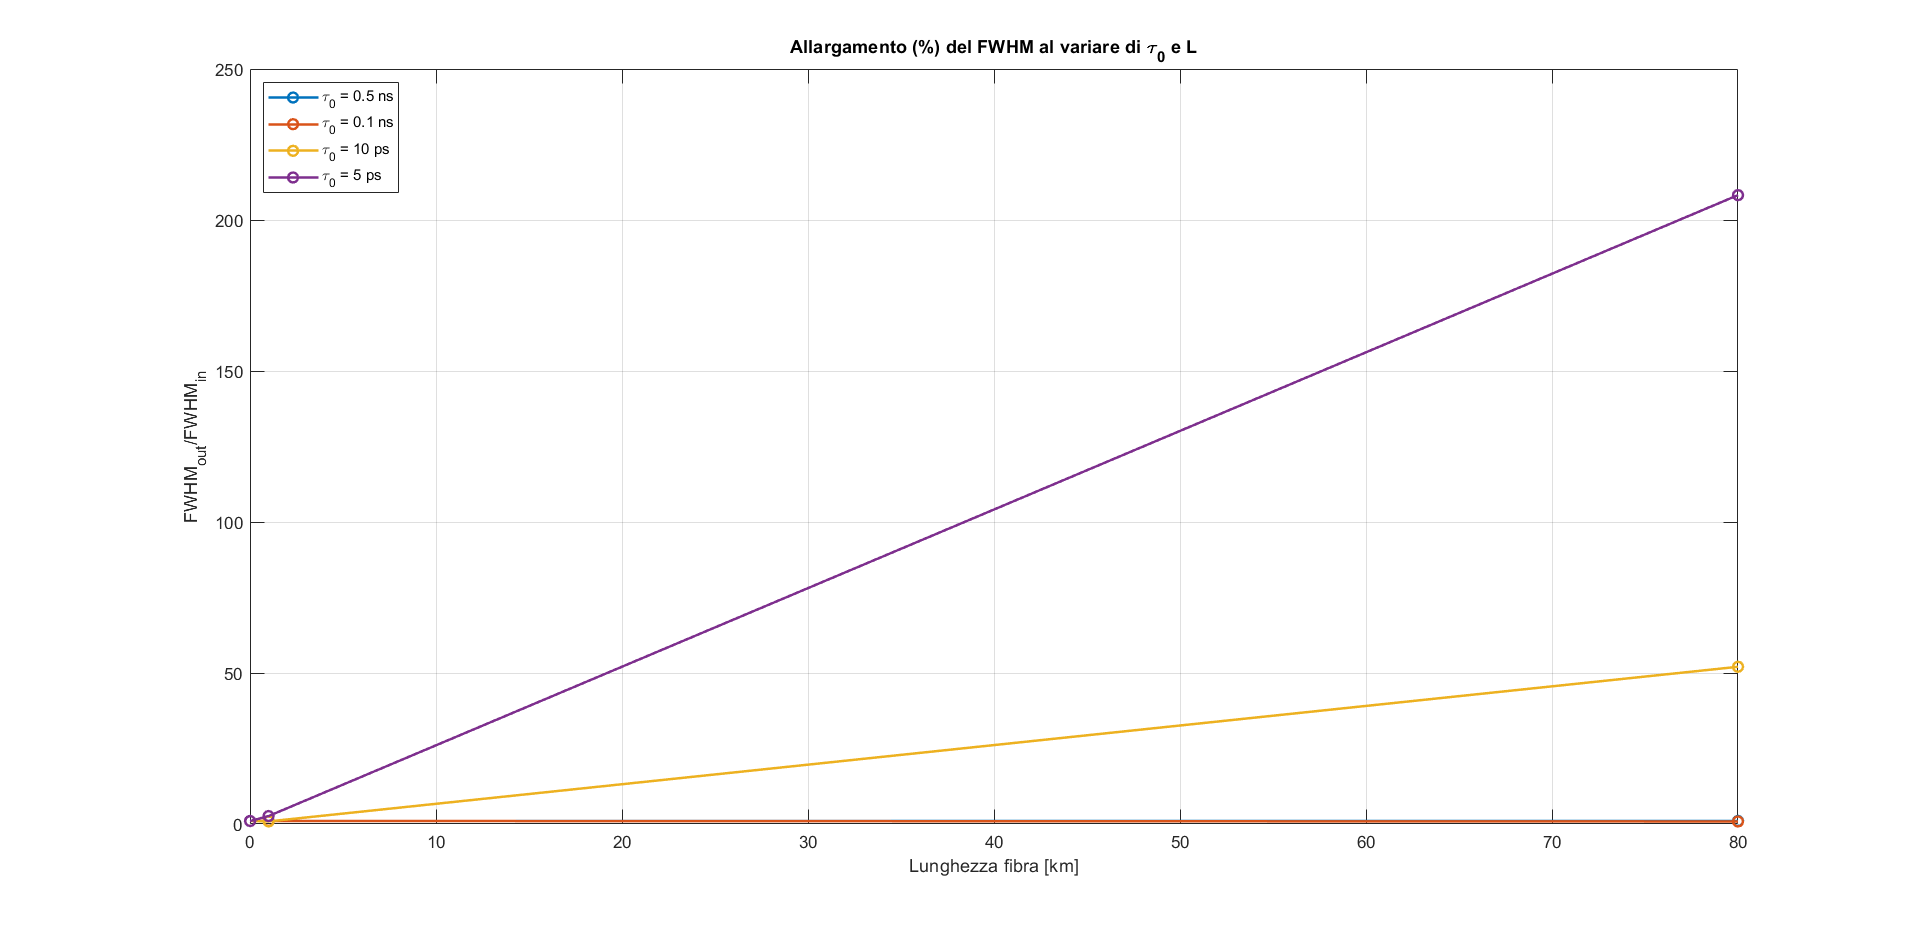
\includegraphics[width=15cm]{lab1/Images/prob2/FWHM_ratio.png}
  \caption{Rapporto tra FWHM in uscita e FWHM in ingresso}
  \label{fig:FWHM_ratio}
\end{figure}

\subsection{Risoluzione temporale e gestione della finestra temporale}
Durante la simulazione numerica degli impulsi nel dominio del tempo, si è presentata una sfida computazionale dovuta al compromesso tra la risoluzione temporale ($\Delta t$)
e l'ampiezza della finestra temporale totale ($T_{\text{tot}}$).
\noindent\\ \\Per rappresentare accuratamente le forme d'onda degli impulsi più stretti ($\tau_0 = 5\,\text{ps}$) senza introdurre distorsioni da campionamento, è
richiesta una risoluzione temporale nell'ordine del sub-picosecondo ($\Delta t \approx 60\,\text{fs}$).

\noindent\\ Tuttavia, considerando una lunghezza di fibra pari a $L = 80\,\text{km}$, il ritardo di gruppo introdotto dal termine del primo ordine
$\beta_1 = \frac{d\beta}{d\omega}$ risulta essere nell'ordine di $\tau_g \approx 390\,\mu\text{s}$. 

\noindent\\ Se si volesse osservare direttamente tale ritardo mantenendo la risoluzione elevata di $60\,\text{fs}$ su una finestra temporale di circa $800\,\mu\text{s}$, il vettore temporale richiederebbe:
\begin{equation}
    N = \frac{T_{\text{tot}}}{\Delta t} \approx \frac{800 \times 10^{-6}}{60 \times 10^{-15}} \approx 1.33 \times 10^{10} \,\,\, \text{punti}
\end{equation}

\noindent Un numero di elementi di questa portata comporta un'occupazione di memoria superiore a $100\,\text{GB}$, rendendo l'elaborazione computazionalmente inattuabile in ambiente MATLAB.

\noindent Per ovviare a questo problema, la simulazione è stata suddivisa in due domini temporali distinti:
\begin{itemize}
    \item \textbf{Dominio A (Alta Risoluzione):} Utilizza un passo di campionamento fine ($\Delta t = 60\,\text{fs}$) su una finestra limitata ($T_{\text{end}} = 15\,\text{ns}$, $N = 5 \times 10^5$ punti). Per evitare che l'impulso esca dalla finestra a causa del ritardo accumulato, il calcolo viene effettuato trascurando il termine di ritardo di gruppo $\beta_1$, considerando quindi la costante di propagazione modificata:
    \begin{equation}
        \beta_{\text{nodelay}}(\omega) = \beta_0 + \frac{1}{2}\beta_2\omega^2
    \end{equation}
    In questo modo gli impulsi rimangono centrati attorno all'origine, permettendo di analizzare con elevata precisione la forma d'onda, la dispersione del secondo ordine ($\beta_2$) e l'effetto dell'attenuazione.

    \item \textbf{Dominio B (Ampia Finestra Temporale):} Utilizza una finestra temporale estesa ($T_{\text{end}} = 400\,\mu\text{s}$, $N = 10^7$ punti) associata a una risoluzione più grossolana ($\Delta t = 40\,\text{ps}$). In questo dominio si impiega l'espressione completa di $\beta(\omega)$:
    \begin{equation}
        \beta(\omega) = \beta_0 + \beta_1\omega + \frac{1}{2}\beta_2\omega^2
    \end{equation}
    Ciò consente di valutare e visualizzare correttamente l'entità del ritardo di gruppo $\tau_g$ su lunghe distanze, pur con un dettaglio della forma d'onda inferiore.
\end{itemize}

\noindent\\ I risultati ottenuti nel Dominio B sono riportati in Figura \ref{fig:pout_t_taug}. Dal grafico si evidenzia chiaramente la traslazione temporale subita dagli impulsi
in uscita al variare della lunghezza della fibra $L$: mentre per $L = 1\,\text{m}$ e $L = 10\,\text{m}$ il ritardo è trascurabile sulla scala dei microsecondi,
per $L = 1\,\text{km}$ e $L = 80\,\text{km}$ gli impulsi subiscono un ritardo di gruppo di circa $4.87\,\mu\text{s}$ e $390\,\mu\text{s}$ rispettivamente, in perfetto
accordo con i valori teorici $\tau_g = \beta_1 L = L / v_g$, riportati nella Tabella \ref{tab:tau_g}.

\begin{figure}[!h]
 \centering
 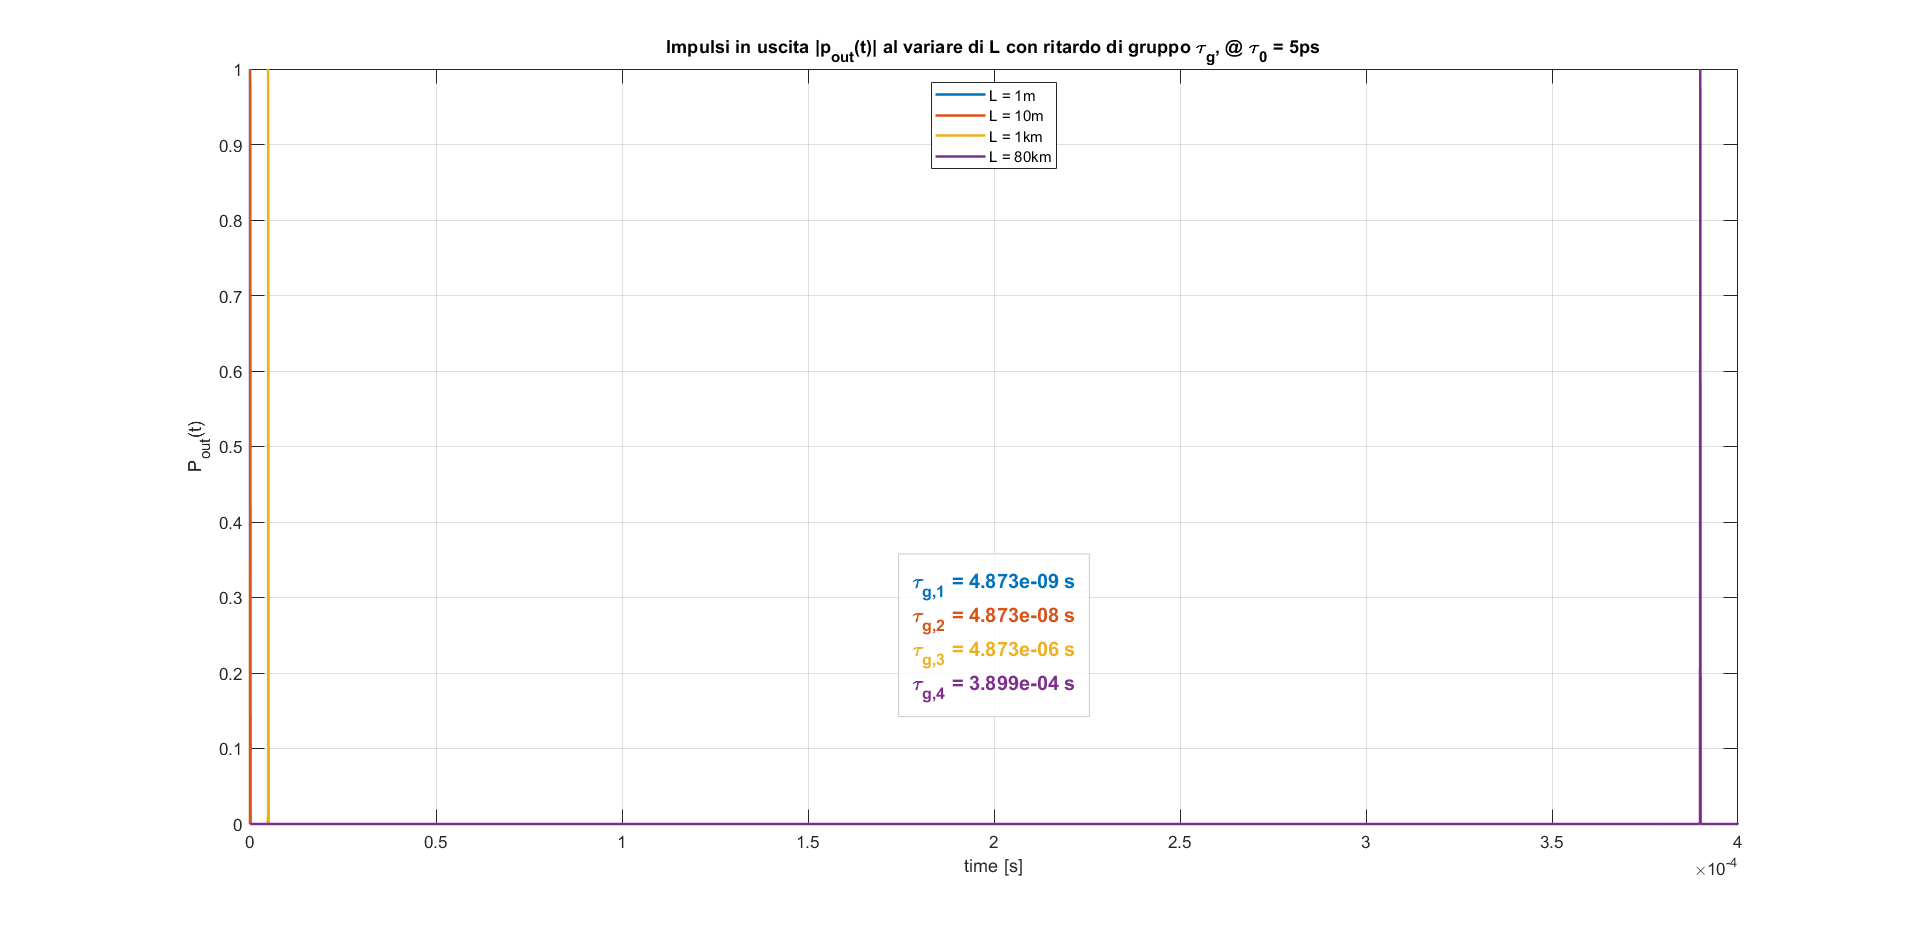
\includegraphics[width=15cm]{lab1/Images/prob2/pout_t_taug.png}
  \caption{Impulsi in uscita includendo il ritardo di gruppo $\tau_g$ al variare di $L$}
  \label{fig:pout_t_taug}
\end{figure}

\begin{table}[!h]
    \centering
    \begin{tabular}{|c|c|}
    \hline
    \textbf{Lunghezza fibra L} & \textbf{Ritardo di gruppo $\boldsymbol{\tau_g}$} \\ \hline \hline
    $1\,m$           & $4.873\,ns$  \\ \hline
    $10\,m$          & $48.73\,ns$  \\ \hline
    $1\,km$          & $4.873\,\mu s$   \\ \hline
    $80\,km$         & $389.9\,\mu s$    \\ \hline
    \end{tabular}
    \caption{Valori dei ritardi di gruppo $\tau_g$ per ciascuna lunghezza della fibra ottica $L$}
    \label{tab:tau_g}
\end{table}

%%%%%%   Terzo esercizio --------------------------------------
\newpage
\section{Biosensore ottico basato su microring in Silicio}
Il terzo assignment del Laboratorio 1 tratta l'utilizzo di un risonatore ad anello in silicio come biosensore, sfruttando il principio dello
spostamento della lunghezza d'onda di risonanza ($\Delta\lambda$) per ricavare informazioni sulla presenza e sulla concentrazione di un analita
depositato su uno strato recettore.

\noindent\\ Il principio fisico alla base del funzionamento è schematizzato in Figura \ref{fig:principio_biosensore}: quando le molecole target (analita) si legano ai recettori immobilizzati sulla superficie del microring, si verifica una variazione locale dell'indice di rifrazione efficace ($n_{\text{eff}}$) della guida d'onda. Tale variazione altera la condizione di risonanza dell'anello, provocando uno shift spettrale $\Delta\lambda$ della risposta in frequenza misurabile all'uscita.

\begin{figure}[!h]
    \centering
    \begin{subfigure}[b]{0.48\textwidth}
        \centering
        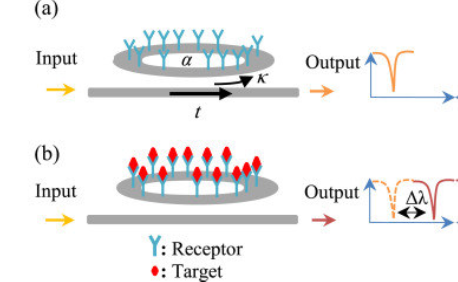
\includegraphics[width=\textwidth]{lab1/Images/prob3/bio_sens.png}
        \caption{Principio di funzionamento con shift $\Delta\lambda$.}
        \label{fig:principio_biosensore}
    \end{subfigure}
    \hfill
    \begin{subfigure}[b]{0.48\textwidth}
        \centering
        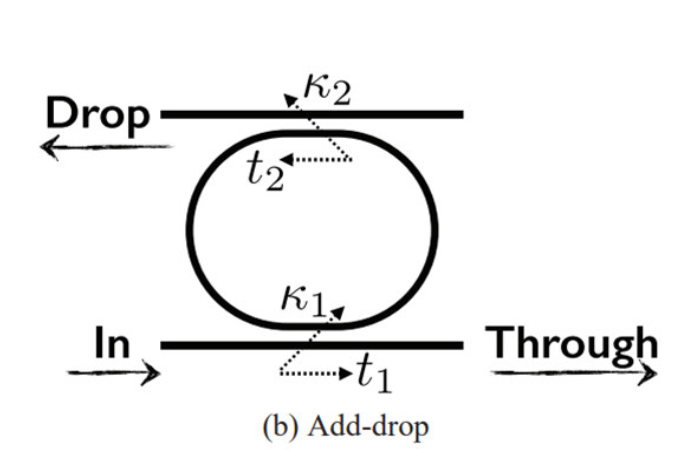
\includegraphics[width=\textwidth]{lab1/Images/prob3/add_drop.png}
        \caption{Schema della configurazione \textit{add-drop}.}
        \label{fig:add_drop}
    \end{subfigure}
    \caption{Principio fisico del biosensore (a) e struttura del microring resonator in configurazione \textit{add-drop} (b).}
    \label{fig:biosensore_e_struttura}
\end{figure}

\noindent La configurazione del microring utilizzata in questo studio è di tipo \textit{add-drop}, mostrata in Figura \ref{fig:add_drop}.
La struttura è composta da un anello risonante accoppiato a due guide d'onda rettilinee (dette \textit{bus waveguides}): 
\begin{itemize}
    \item La guida d'ingresso, che comprende la porta di \textit{Input} (In) e la porta di trasmissione principale (\textit{Through});
    \item La guida di prelievo, contenente la porta di prelievo del segnale risonante (\textit{Drop}).
\end{itemize}

\noindent\\ Questa architettura \textit{add-drop} è caratterizzata dai seguenti parametri fisici ed ottici:
\begin{itemize}
    \item $R = 8 \,\mu m$: raggio del microring;
    \item $L_{rt} = 2\pi R = 16\pi \,\mu m$: lunghezza della circonferenza del risonatore;
    \item $\alpha_{dB} = 0.5 \, \text{dB/cm}$: coefficiente di attenuazione per unità di lunghezza all'interno del ring;
    \item  $\kappa^2 = 0.03 = \kappa_1^2 = \kappa_2^2$: coefficienti di accoppiamento in ampiezza;
    \item $t_1, t_2$: coefficienti di trasmissione in ampiezza delle due regioni di accoppiamento, legati ai coefficienti di accoppiamento dalla relazione di
    conservazione dell'energia $t_i^2 + \kappa_i^2 = 1$ (nel caso di accoppiamento privo di perdite);
    \item $\lambda_0 = 1.55 \,\mu m$: lunghezza d'onda operativa.
\end{itemize}

\noindent\\
\subsection{Spettro di trasmissione alle porte Through e Drop}
Nella prima fase dell'analisi si valuta lo spettro di trasmissione in potenza del risonatore ad anello sia alla porta \textit{Through} sia alla porta \textit{Drop},
ponendo a confronto due differenti valori per il coefficiente di accoppiamento: $k^2 = 0.03$ e $k^2 = 0.3$.

\newpage

\begin{figure}[!h]
 \centering
 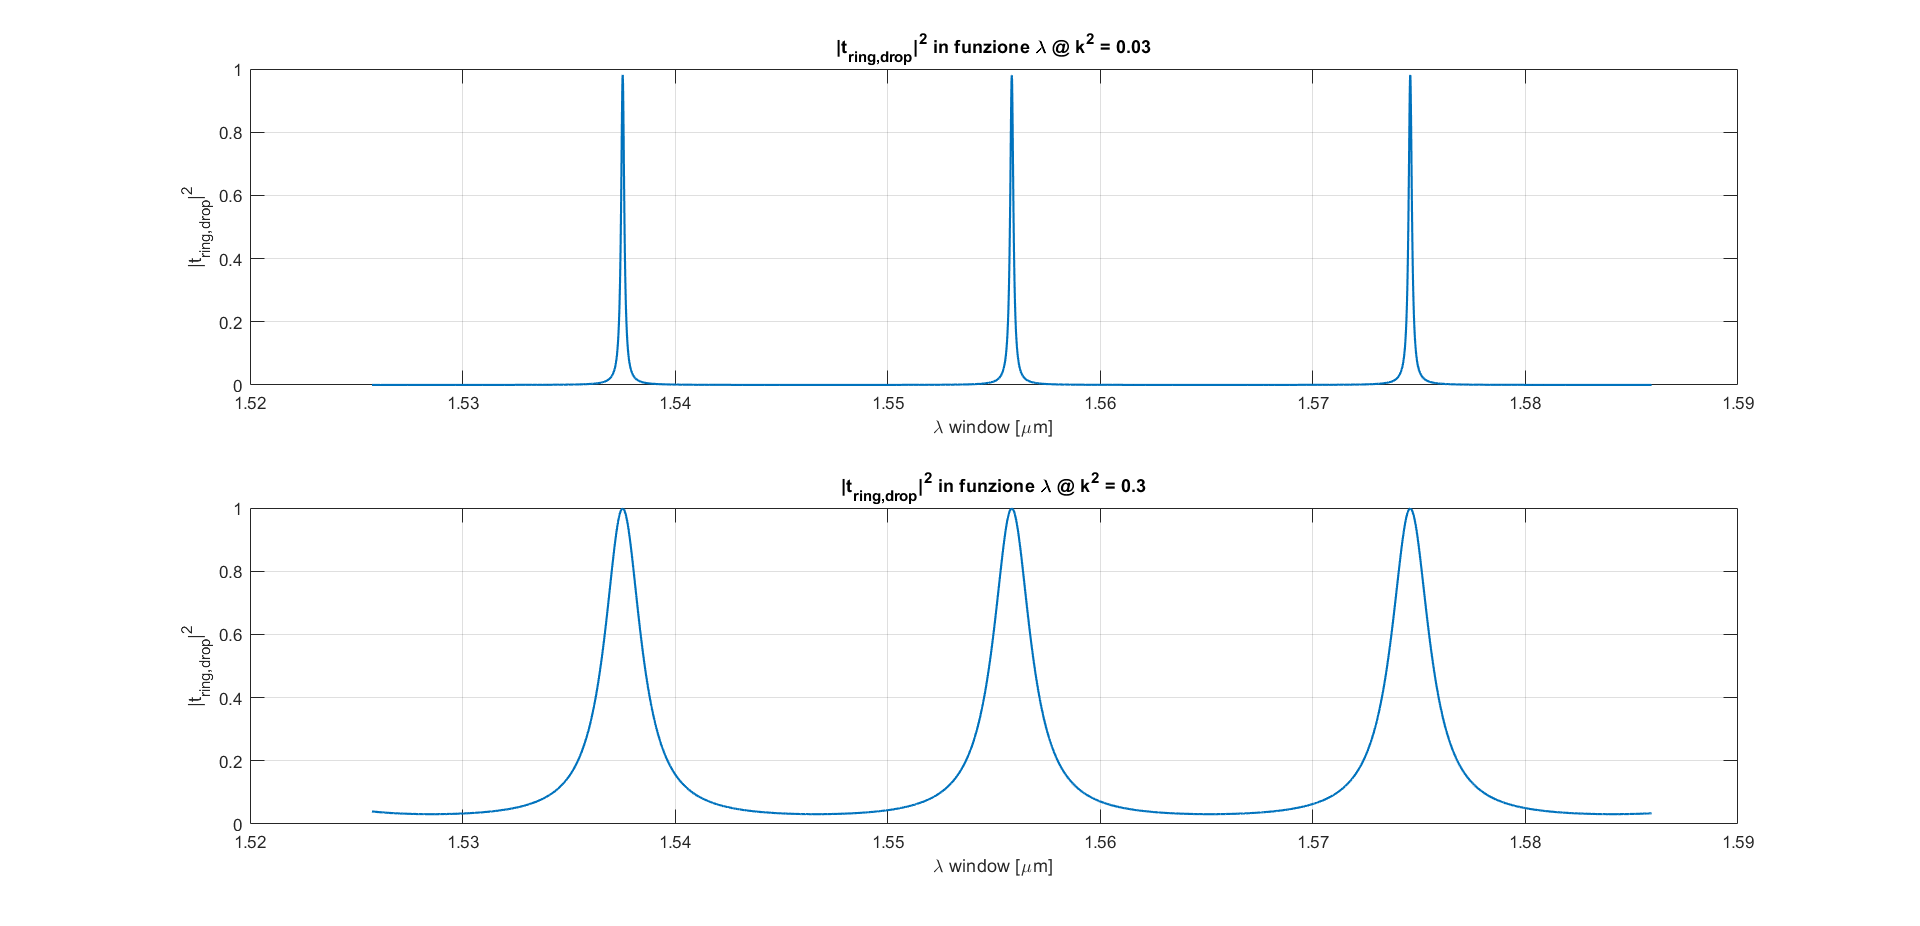
\includegraphics[width=15cm]{lab1/Images/prob3/t_drop.png}
  \caption{Spettro di trasmissione in potenza alla porta \textit{Drop} per $k^2 = 0.03$ e $k^2 = 0.3$}
  \label{fig:t_drop}
\end{figure}

\begin{figure}[!h]
 \centering
 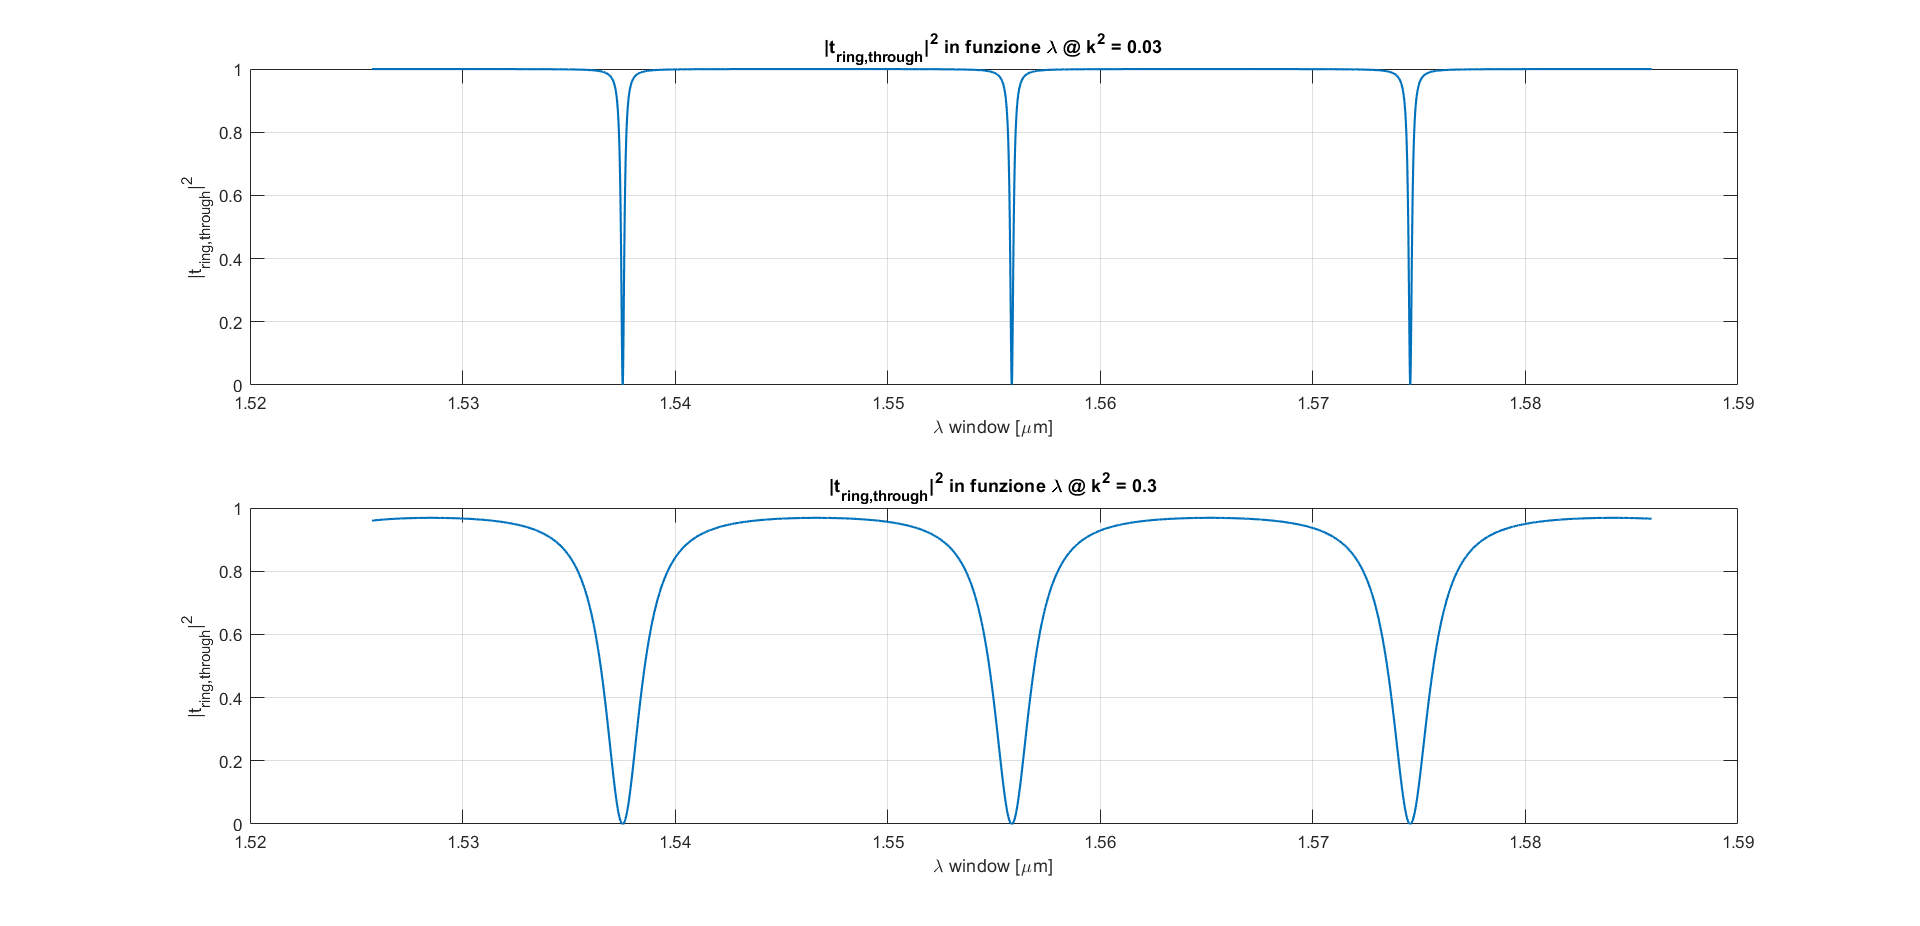
\includegraphics[width=15cm]{lab1/Images/prob3/t_thru.png}
  \caption{Spettro di trasmissione in potenza alla porta \textit{Through} per $k^2 = 0.03$ e $k^2 = 0.3$}
  \label{fig:t_thru}
\end{figure}

\noindent Analizzando le risposte spettrali riportate nelle Figure \ref{fig:t_drop} e \ref{fig:t_thru}, si osserva che un valore più elevato del coefficiente di accoppiamento ($k^2$)
aumenta la potenza accoppiata verso le guide rettilinee, riducendo l'ampiezza del campo elettrico risonante all'interno dell'anello. Questo si traduce in un
aumento della larghezza a mezza altezza ($\text{FWHM}$) e in una conseguente riduzione del fattore di qualità ($Q$).

\noindent\\ Ai fini dell'applicazione come biosensore, la condizione ottimale richiede un picco di risonanza con una $\text{FWHM}$ il più stretta possibile, così da garantire la
massima accuratezza nella determinazione della lunghezza d'onda di risonanza e nell'individuazione dei minimi shift spettrali. Di conseguenza, la configurazione migliore
è quella con $k^2 = 0.03$.

\noindent\\ La presenza dell'analita depositato sullo strato recettore induce una variazione dell'indice di rifrazione efficace ($\Delta n_{\text{eff}}$), provocando uno
shift spettrale della lunghezza d'onda di risonanza pari a:
\begin{equation}
    \Delta\lambda = \Gamma_{\text{clad}} \Delta n_{\text{clad}} \frac{\lambda_0}{n_{\text{eff,0}}}
\end{equation}
Oltre alla variazione dell'indice di rifrazione, l'analita introduce un ulteriore termine di perdita all'interno della cavità risonante. L'impatto dettagliato di tali
perdite aggiuntive sulla risposta del sensore verrà analizzato nella sottosezione seguente.

\subsection{Introduzione dell'analita e calcolo di Q}
Si procede quindi ad analizzare il comportamento del risonatore ad anello in presenza dell'analita, che comporta l'aggiunta di ulteriore termine di perdita $\alpha_{analyte}$,
che varia in un range compreso tra $0$ e $30 cm^{-1}$. Di conseguenza, le perdite totali $\alpha_{tot}$ all'interno del risonatore diventano:
\begin{equation}
    a_{tot} = \sqrt{e^{-(\Gamma_{clad}\alpha_{analyte} + \alpha)\cdot L_{rt}}}
\end{equation}

\noindent Si è quindi proceduto con il calcolo del fattore di qualità $Q$, considerando tre differenti valori di $\Gamma_{clad}$, ossia $2\%$, $6\%$ e $15\%$.
Il fattore di qualità $Q$ è stato calcolato come:
\begin{equation}
    Q = \frac{\lambda_m}{\text{FWHM}}
\end{equation}

\noindent dove:
\begin{equation}
    \text{FWHM} = \frac{(1-t^2a_{tot})\lambda_m^2}{\pi n_g L_{rt} \sqrt{t^2 a_{tot}}}
\end{equation}

\noindent e $\lambda_m$ è la lunghezza d'onda di risonanza più prossima a quella operativa $\lambda_0$.

\noindent\\ In Figura \ref{fig:Q_vs_a} è riportato l'andamento del fattore di qualità $Q$ al variare di $\alpha_{analyte}$, per i tre differenti valori di $\Gamma_{clad}$
precedentemente illustrati e considerando sia $k^2 = 0.03$ che $k^2 = 0.3$.

\begin{figure}[!h]
 \centering
 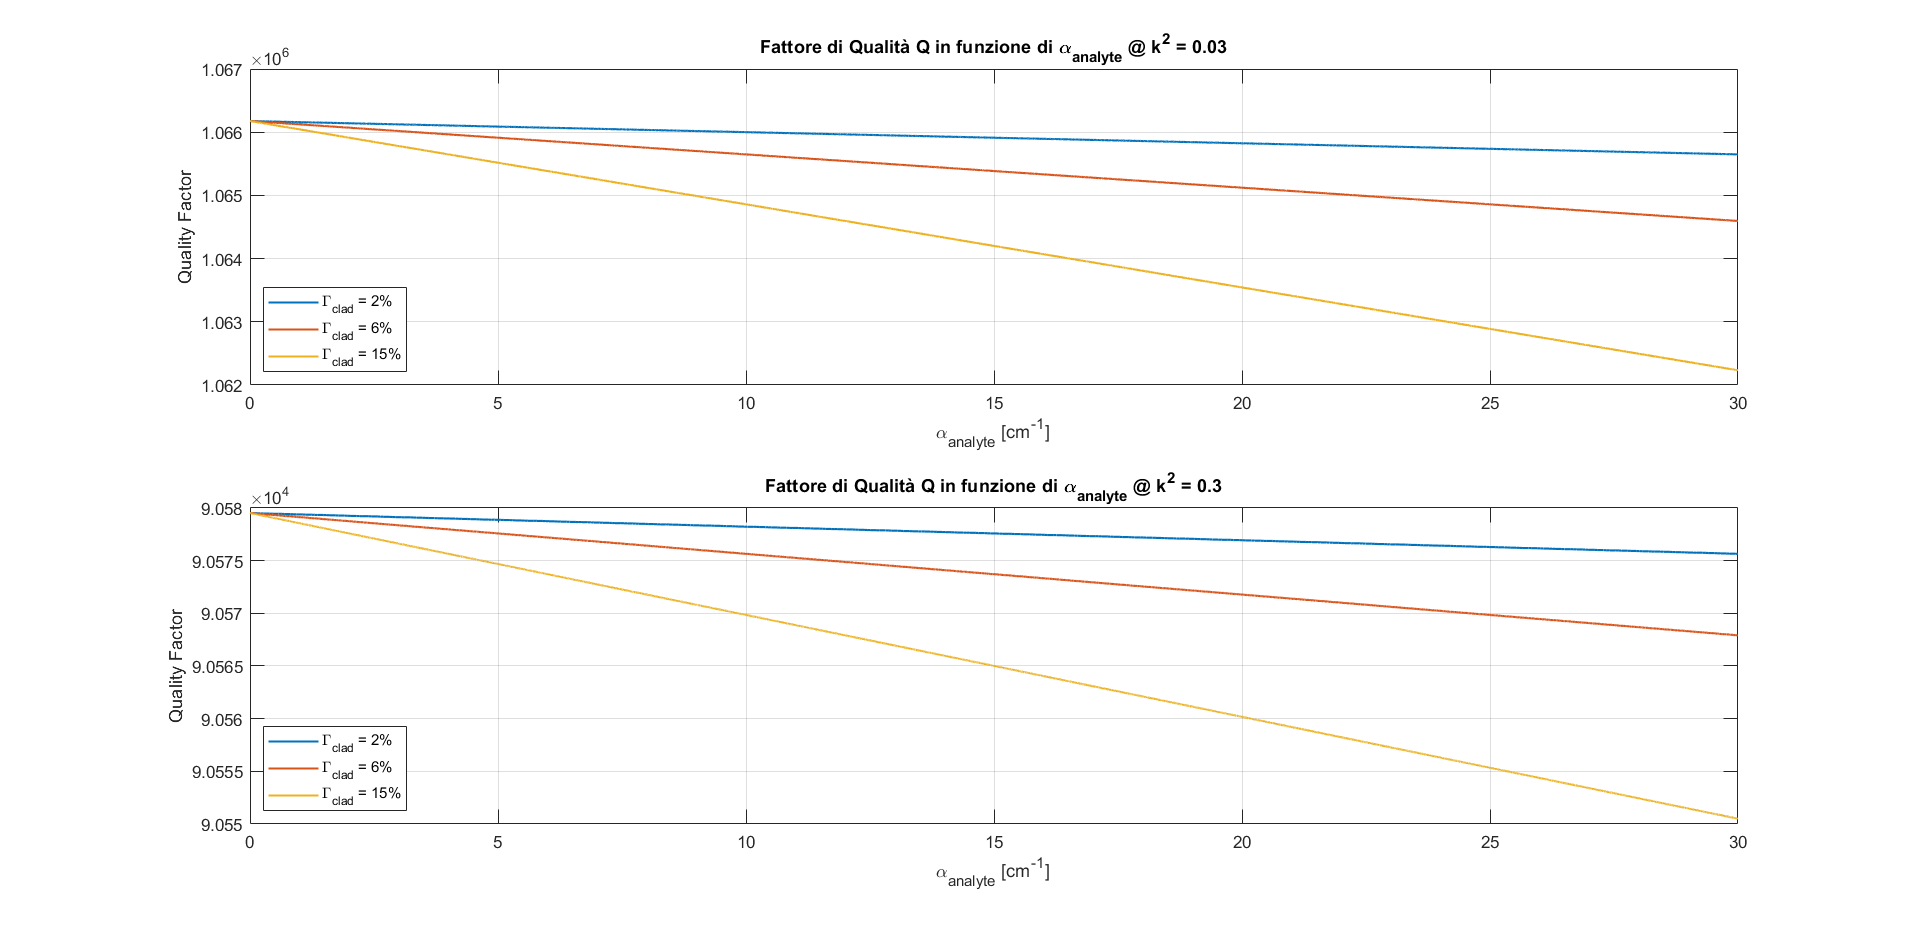
\includegraphics[width=15cm]{lab1/Images/prob3/Q_vs_a.png}
  \caption{Fattore di qualità Q al variare di $\alpha_{analyte}$ per tre differenti valori di $\Gamma_{clad}$}
  \label{fig:Q_vs_a}
\end{figure}

\noindent Dalla Figura riportata sopra è evidente come il fattore di qualità $\text{Q}$ diminuisca all'aumentare delle perdite introdotte dall'analita, con un andamento più marcato
per valori più elevati di $\Gamma_{clad}$. Inoltre, si può notare come un valore più elevato del coefficiente di accoppiamento $k^2$, a cui corrisponde una $\text{FWHM}$ maggiore,
comporti un fattore di qualità inferiore di più di un ordine di grandezza, confermando quanto osservato nella sottosezione precedente.

\subsection{Calcolo della Sensitivity $\boldsymbol{S}$ e del Detection Limit $\boldsymbol{DL}$}
Infine, si è proceduto con il calcolo della sensibilità ($S$, \textit{Sensitivity}) e del limite di rilevabilità ($DL$, \textit{Detection Limit}) del biosensore, considerando
i tre differenti valori di $\Gamma_{\text{clad}}$ e un coefficiente di accoppiamento pari a $k^2 = 0.03$.

\noindent\\ La sensibilità $S$ rappresenta la variazione della lunghezza d'onda di risonanza rispetto alla variazione dell'indice di rifrazione dell'analita ed è definita come:
\begin{equation}
    S = \frac{\Delta\lambda}{\Delta n_{\text{clad}}} = \Gamma_{\text{clad}} \frac{\lambda_0}{n_{\text{eff,0}}}
\end{equation}

\noindent Il limite di rilevabilità $DL$ quantifica invece la minima variazione di indice di rifrazione percepibile dal sistema ed è espresso in funzione della sensibilità $S$
e del fattore di qualità $Q$:
\begin{equation}
    DL = \frac{\lambda_0}{Q \cdot S}
\end{equation}

\noindent In termini di prestazioni, un biosensore ideale richiede un valore di sensibilità $S$ elevato (in modo da massimizzare lo shift spettrale $\Delta\lambda$ a parità di analita)
e un limite di rilevabilità $DL$ il più basso possibile (per poter identificare concentrazioni infinitesimali di analita). Di conseguenza, per ottimizzare il dispositivo è
necessario disporre di un fattore di qualità $Q$ e di una sensibilità $S$ entrambi elevati.

\noindent\\ L'andamento di $S$ in funzione di $\Gamma_{\text{clad}}$ è riportato in Figura \ref{fig:S}, mentre l'andamento di $DL$ al variare di $\alpha_{\text{analyte}}$ per i diversi
valori di $\Gamma_{\text{clad}}$ è mostrato in Figura \ref{fig:DL}.

\begin{figure}[!h]
 \centering
 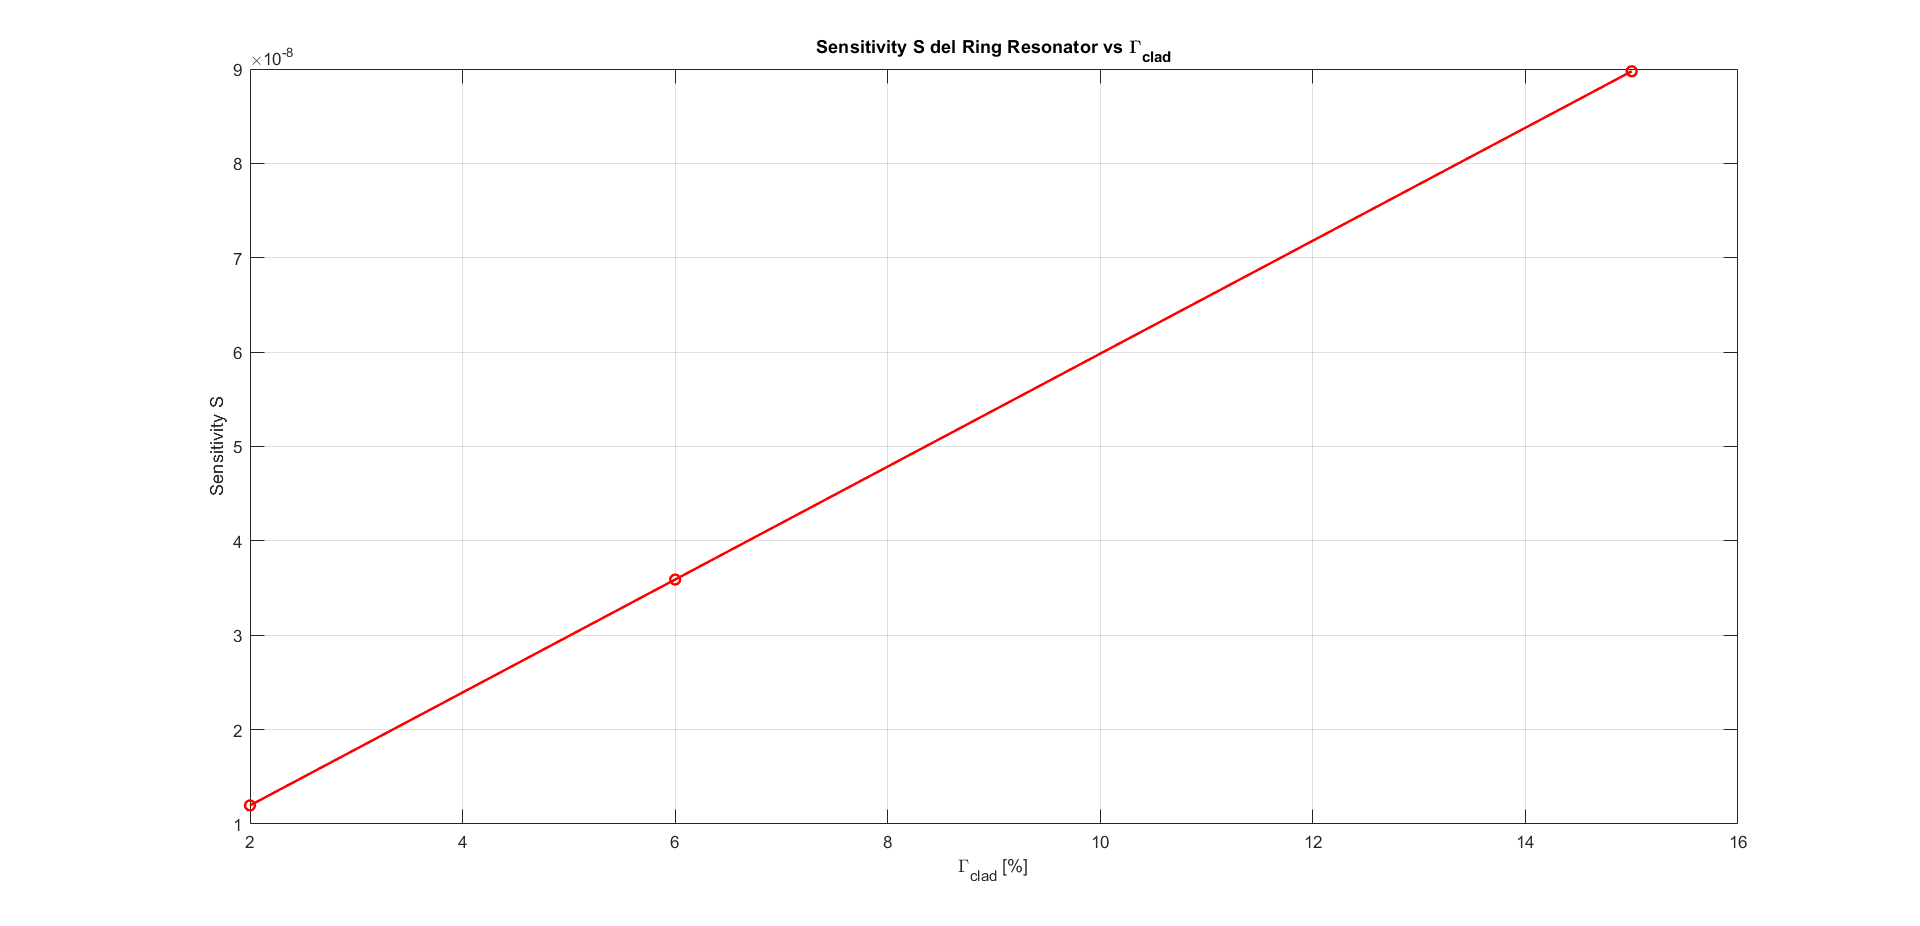
\includegraphics[width=12.5cm]{lab1/Images/prob3/S.png}
  \caption{Andamento della sensibilità $S$ in funzione di $\Gamma_{\text{clad}}$.}
  \label{fig:S}
\end{figure}

\begin{figure}[!h]
 \centering
 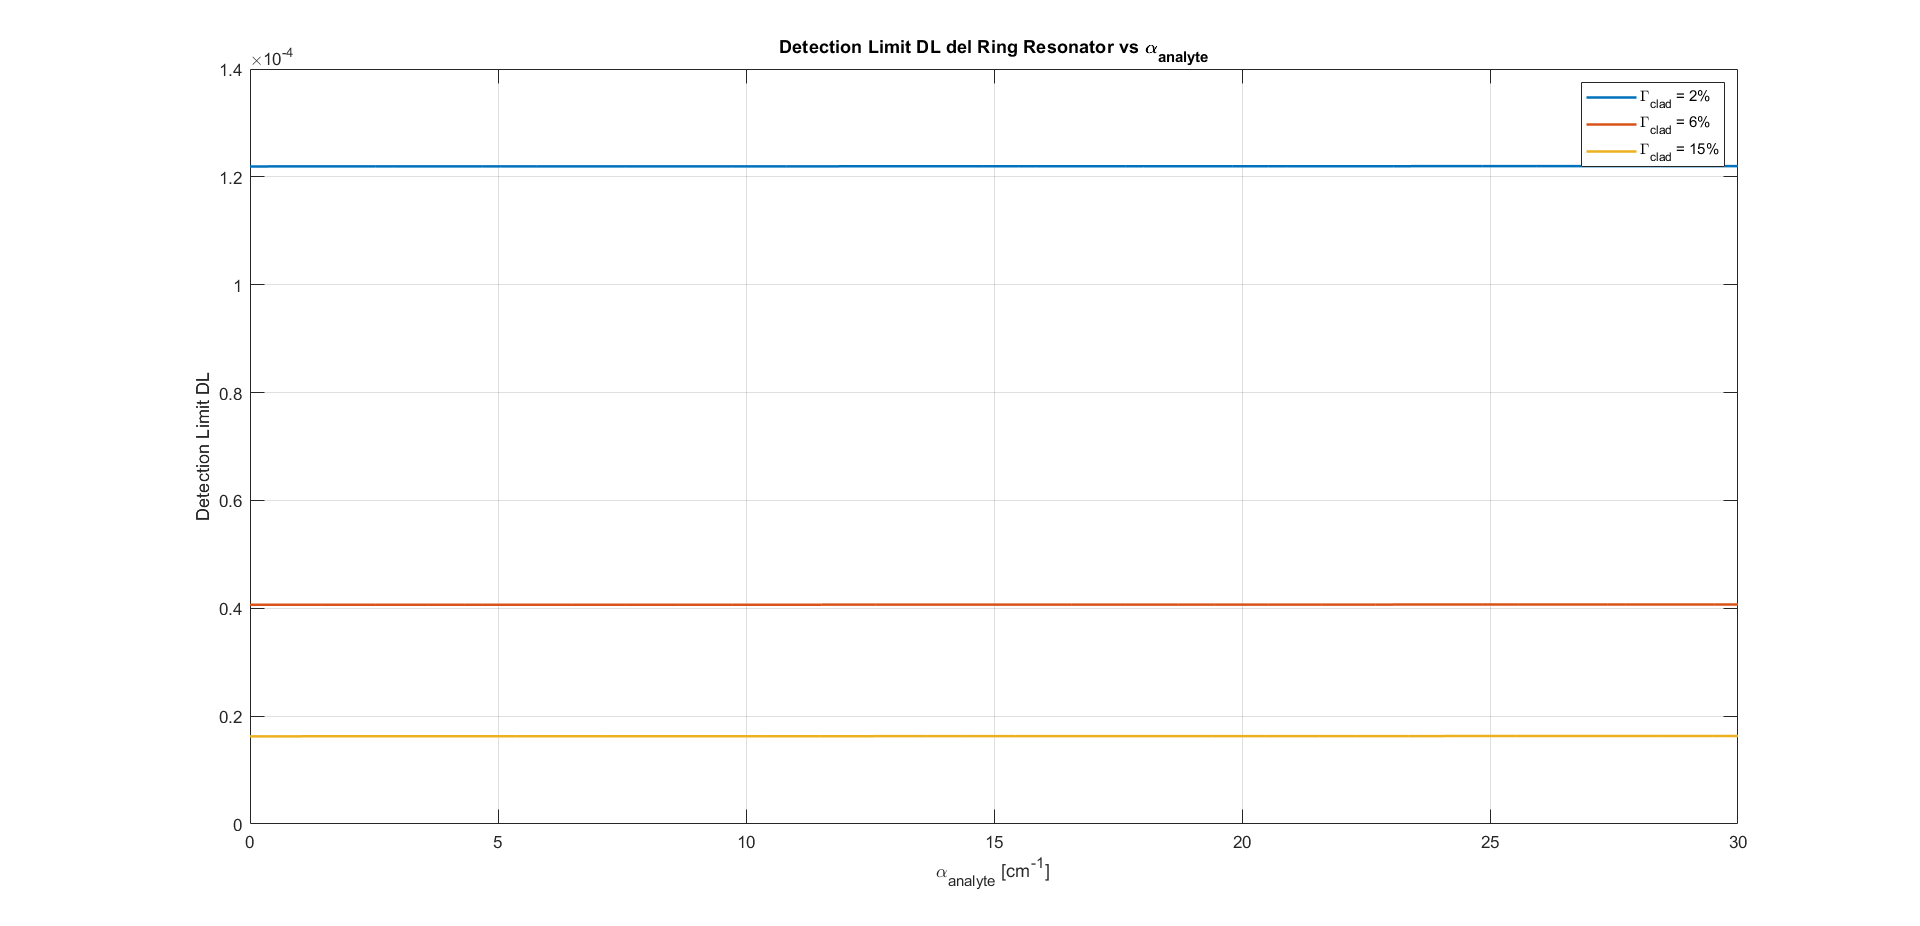
\includegraphics[width=12.5cm]{lab1/Images/prob3/DL.png}
  \caption{Andamento del limite di rilevabilità $DL$ in funzione di $\alpha_{\text{analyte}}$ al variare di $\Gamma_{\text{clad}}$.}
  \label{fig:DL}
\end{figure}

\noindent Analizzando i risultati ottenuti si possono trarre le seguenti considerazioni sulle prestazioni del sensore:
\begin{itemize}
    \item \textbf{Dipendenza da $\alpha_{\text{analyte}}$:} Al crescere delle perdite per assorbimento introdotte dall'analita, la sensibilità $S$ rimane costante poiché
    dipende unicamente dai parametri geometrici e dal confinamento $\Gamma_{\text{clad}}$. Tuttavia, l'incremento di $\alpha_{\text{analyte}}$ provoca un degrado del
    fattore di qualità $Q$, determinando un aumento (peggioramento) del limite di rilevabilità $DL$. Nel grafico sopra riportato, l'andamento di $DL$ risulta pressoché costante
    in quanto la variazione di $Q$ indotta dall'analita è estremamente ridotta e visivamente non apprezzabile nella scala del grafico.
    
    \item \textbf{Dipendenza da $\Gamma_{\text{clad}}$ e Trade-off prestazionale:} L'aumento di $\Gamma_{\text{clad}}$ incrementa linearmente la sensibilità $S$, portando a
    una maggiore interazione del campo con l'analita. Sebbene un $\Gamma_{\text{clad}}$ più elevato riduca il fattore di qualità $Q$ a causa delle maggiori perdite,
    l'incremento di $S$ risulta dominante nel bilancio di $DL$, determinando una riduzione netta (miglioramento) del limite di rilevabilità. Si individua così un chiaro
    \textit{trade-off} progettuale: massimizzare $\Gamma_{\text{clad}}$ permette di ottimizzare la sensibilità e ridurre il $DL$, accettando al contempo una riduzione della
    selettività spettrale dovuta al calo del fattore $Q$.
\end{itemize}